% Options for packages loaded elsewhere
\PassOptionsToPackage{unicode}{hyperref}
\PassOptionsToPackage{hyphens}{url}
%
\documentclass[
]{article}
\usepackage{amsmath,amssymb}
\usepackage{iftex}
\ifPDFTeX
  \usepackage[T1]{fontenc}
  \usepackage[utf8]{inputenc}
  \usepackage{textcomp} % provide euro and other symbols
\else % if luatex or xetex
  \usepackage{unicode-math} % this also loads fontspec
  \defaultfontfeatures{Scale=MatchLowercase}
  \defaultfontfeatures[\rmfamily]{Ligatures=TeX,Scale=1}
\fi
\usepackage{lmodern}
\ifPDFTeX\else
  % xetex/luatex font selection
\fi
% Use upquote if available, for straight quotes in verbatim environments
\IfFileExists{upquote.sty}{\usepackage{upquote}}{}
\IfFileExists{microtype.sty}{% use microtype if available
  \usepackage[]{microtype}
  \UseMicrotypeSet[protrusion]{basicmath} % disable protrusion for tt fonts
}{}
\makeatletter
\@ifundefined{KOMAClassName}{% if non-KOMA class
  \IfFileExists{parskip.sty}{%
    \usepackage{parskip}
  }{% else
    \setlength{\parindent}{0pt}
    \setlength{\parskip}{6pt plus 2pt minus 1pt}}
}{% if KOMA class
  \KOMAoptions{parskip=half}}
\makeatother
\usepackage{xcolor}
\usepackage[margin=1in]{geometry}
\usepackage{color}
\usepackage{fancyvrb}
\newcommand{\VerbBar}{|}
\newcommand{\VERB}{\Verb[commandchars=\\\{\}]}
\DefineVerbatimEnvironment{Highlighting}{Verbatim}{commandchars=\\\{\}}
% Add ',fontsize=\small' for more characters per line
\usepackage{framed}
\definecolor{shadecolor}{RGB}{248,248,248}
\newenvironment{Shaded}{\begin{snugshade}}{\end{snugshade}}
\newcommand{\AlertTok}[1]{\textcolor[rgb]{0.94,0.16,0.16}{#1}}
\newcommand{\AnnotationTok}[1]{\textcolor[rgb]{0.56,0.35,0.01}{\textbf{\textit{#1}}}}
\newcommand{\AttributeTok}[1]{\textcolor[rgb]{0.13,0.29,0.53}{#1}}
\newcommand{\BaseNTok}[1]{\textcolor[rgb]{0.00,0.00,0.81}{#1}}
\newcommand{\BuiltInTok}[1]{#1}
\newcommand{\CharTok}[1]{\textcolor[rgb]{0.31,0.60,0.02}{#1}}
\newcommand{\CommentTok}[1]{\textcolor[rgb]{0.56,0.35,0.01}{\textit{#1}}}
\newcommand{\CommentVarTok}[1]{\textcolor[rgb]{0.56,0.35,0.01}{\textbf{\textit{#1}}}}
\newcommand{\ConstantTok}[1]{\textcolor[rgb]{0.56,0.35,0.01}{#1}}
\newcommand{\ControlFlowTok}[1]{\textcolor[rgb]{0.13,0.29,0.53}{\textbf{#1}}}
\newcommand{\DataTypeTok}[1]{\textcolor[rgb]{0.13,0.29,0.53}{#1}}
\newcommand{\DecValTok}[1]{\textcolor[rgb]{0.00,0.00,0.81}{#1}}
\newcommand{\DocumentationTok}[1]{\textcolor[rgb]{0.56,0.35,0.01}{\textbf{\textit{#1}}}}
\newcommand{\ErrorTok}[1]{\textcolor[rgb]{0.64,0.00,0.00}{\textbf{#1}}}
\newcommand{\ExtensionTok}[1]{#1}
\newcommand{\FloatTok}[1]{\textcolor[rgb]{0.00,0.00,0.81}{#1}}
\newcommand{\FunctionTok}[1]{\textcolor[rgb]{0.13,0.29,0.53}{\textbf{#1}}}
\newcommand{\ImportTok}[1]{#1}
\newcommand{\InformationTok}[1]{\textcolor[rgb]{0.56,0.35,0.01}{\textbf{\textit{#1}}}}
\newcommand{\KeywordTok}[1]{\textcolor[rgb]{0.13,0.29,0.53}{\textbf{#1}}}
\newcommand{\NormalTok}[1]{#1}
\newcommand{\OperatorTok}[1]{\textcolor[rgb]{0.81,0.36,0.00}{\textbf{#1}}}
\newcommand{\OtherTok}[1]{\textcolor[rgb]{0.56,0.35,0.01}{#1}}
\newcommand{\PreprocessorTok}[1]{\textcolor[rgb]{0.56,0.35,0.01}{\textit{#1}}}
\newcommand{\RegionMarkerTok}[1]{#1}
\newcommand{\SpecialCharTok}[1]{\textcolor[rgb]{0.81,0.36,0.00}{\textbf{#1}}}
\newcommand{\SpecialStringTok}[1]{\textcolor[rgb]{0.31,0.60,0.02}{#1}}
\newcommand{\StringTok}[1]{\textcolor[rgb]{0.31,0.60,0.02}{#1}}
\newcommand{\VariableTok}[1]{\textcolor[rgb]{0.00,0.00,0.00}{#1}}
\newcommand{\VerbatimStringTok}[1]{\textcolor[rgb]{0.31,0.60,0.02}{#1}}
\newcommand{\WarningTok}[1]{\textcolor[rgb]{0.56,0.35,0.01}{\textbf{\textit{#1}}}}
\usepackage{longtable,booktabs,array}
\usepackage{calc} % for calculating minipage widths
% Correct order of tables after \paragraph or \subparagraph
\usepackage{etoolbox}
\makeatletter
\patchcmd\longtable{\par}{\if@noskipsec\mbox{}\fi\par}{}{}
\makeatother
% Allow footnotes in longtable head/foot
\IfFileExists{footnotehyper.sty}{\usepackage{footnotehyper}}{\usepackage{footnote}}
\makesavenoteenv{longtable}
\usepackage{graphicx}
\makeatletter
\def\maxwidth{\ifdim\Gin@nat@width>\linewidth\linewidth\else\Gin@nat@width\fi}
\def\maxheight{\ifdim\Gin@nat@height>\textheight\textheight\else\Gin@nat@height\fi}
\makeatother
% Scale images if necessary, so that they will not overflow the page
% margins by default, and it is still possible to overwrite the defaults
% using explicit options in \includegraphics[width, height, ...]{}
\setkeys{Gin}{width=\maxwidth,height=\maxheight,keepaspectratio}
% Set default figure placement to htbp
\makeatletter
\def\fps@figure{htbp}
\makeatother
\setlength{\emergencystretch}{3em} % prevent overfull lines
\providecommand{\tightlist}{%
  \setlength{\itemsep}{0pt}\setlength{\parskip}{0pt}}
\setcounter{secnumdepth}{-\maxdimen} % remove section numbering
\usepackage{booktabs}
\usepackage{longtable}
\usepackage{array}
\usepackage{multirow}
\usepackage{wrapfig}
\usepackage{float}
\usepackage{colortbl}
\usepackage{pdflscape}
\usepackage{tabu}
\usepackage{threeparttable}
\usepackage{threeparttablex}
\usepackage[normalem]{ulem}
\usepackage{makecell}
\usepackage{xcolor}
\ifLuaTeX
  \usepackage{selnolig}  % disable illegal ligatures
\fi
\usepackage{bookmark}
\IfFileExists{xurl.sty}{\usepackage{xurl}}{} % add URL line breaks if available
\urlstyle{same}
\hypersetup{
  pdftitle={Causalness, frequency, diachrony and the causal-noncausal alternation in Italian and Spanish},
  pdfauthor={Giulia Mazzola (Newcastle University) and Guglielmo Inglese (Università di Torino)},
  hidelinks,
  pdfcreator={LaTeX via pandoc}}

\title{Causalness, frequency, diachrony and the causal-noncausal
alternation in Italian and Spanish}
\author{Giulia Mazzola (Newcastle University) and Guglielmo Inglese
(Università di Torino)}
\date{April 2025}

\begin{document}
\maketitle

\begin{Shaded}
\begin{Highlighting}[]
\CommentTok{\# List of required packages}
\NormalTok{packages }\OtherTok{\textless{}{-}} \FunctionTok{c}\NormalTok{(}
  \StringTok{"tidyverse"}\NormalTok{, }\StringTok{"knitr"}\NormalTok{, }\StringTok{"data.table"}\NormalTok{, }\StringTok{"DT"}\NormalTok{, }\StringTok{"here"}\NormalTok{, }\StringTok{"kableExtra"}\NormalTok{,}
  \StringTok{"lme4"}\NormalTok{, }\StringTok{"openxlsx"}\NormalTok{, }\StringTok{"readxl"}\NormalTok{, }\StringTok{"wesanderson"}\NormalTok{, }\StringTok{"stringr"}\NormalTok{,}
  \StringTok{"itsadug"}\NormalTok{, }\StringTok{"mgcv"}\NormalTok{, }\StringTok{"report"}\NormalTok{, }\StringTok{"gratia"}
\NormalTok{)}

\CommentTok{\# Install any packages not already installed}
\NormalTok{installed\_packages }\OtherTok{\textless{}{-}} \FunctionTok{rownames}\NormalTok{(}\FunctionTok{installed.packages}\NormalTok{())}
\NormalTok{to\_install }\OtherTok{\textless{}{-}} \FunctionTok{setdiff}\NormalTok{(packages, installed\_packages)}

\ControlFlowTok{if}\NormalTok{ (}\FunctionTok{length}\NormalTok{(to\_install) }\SpecialCharTok{\textgreater{}} \DecValTok{0}\NormalTok{) \{}
  \FunctionTok{install.packages}\NormalTok{(to\_install)}
\NormalTok{\}}

\CommentTok{\# Load the packages}
\FunctionTok{lapply}\NormalTok{(packages, library, }\AttributeTok{character.only =} \ConstantTok{TRUE}\NormalTok{)}
\end{Highlighting}
\end{Shaded}

\begin{verbatim}
## [[1]]
##  [1] "lubridate" "forcats"   "stringr"   "dplyr"     "purrr"     "readr"    
##  [7] "tidyr"     "tibble"    "ggplot2"   "tidyverse" "stats"     "graphics" 
## [13] "grDevices" "utils"     "datasets"  "methods"   "base"     
## 
## [[2]]
##  [1] "knitr"     "lubridate" "forcats"   "stringr"   "dplyr"     "purrr"    
##  [7] "readr"     "tidyr"     "tibble"    "ggplot2"   "tidyverse" "stats"    
## [13] "graphics"  "grDevices" "utils"     "datasets"  "methods"   "base"     
## 
## [[3]]
##  [1] "data.table" "knitr"      "lubridate"  "forcats"    "stringr"   
##  [6] "dplyr"      "purrr"      "readr"      "tidyr"      "tibble"    
## [11] "ggplot2"    "tidyverse"  "stats"      "graphics"   "grDevices" 
## [16] "utils"      "datasets"   "methods"    "base"      
## 
## [[4]]
##  [1] "DT"         "data.table" "knitr"      "lubridate"  "forcats"   
##  [6] "stringr"    "dplyr"      "purrr"      "readr"      "tidyr"     
## [11] "tibble"     "ggplot2"    "tidyverse"  "stats"      "graphics"  
## [16] "grDevices"  "utils"      "datasets"   "methods"    "base"      
## 
## [[5]]
##  [1] "here"       "DT"         "data.table" "knitr"      "lubridate" 
##  [6] "forcats"    "stringr"    "dplyr"      "purrr"      "readr"     
## [11] "tidyr"      "tibble"     "ggplot2"    "tidyverse"  "stats"     
## [16] "graphics"   "grDevices"  "utils"      "datasets"   "methods"   
## [21] "base"      
## 
## [[6]]
##  [1] "kableExtra" "here"       "DT"         "data.table" "knitr"     
##  [6] "lubridate"  "forcats"    "stringr"    "dplyr"      "purrr"     
## [11] "readr"      "tidyr"      "tibble"     "ggplot2"    "tidyverse" 
## [16] "stats"      "graphics"   "grDevices"  "utils"      "datasets"  
## [21] "methods"    "base"      
## 
## [[7]]
##  [1] "lme4"       "Matrix"     "kableExtra" "here"       "DT"        
##  [6] "data.table" "knitr"      "lubridate"  "forcats"    "stringr"   
## [11] "dplyr"      "purrr"      "readr"      "tidyr"      "tibble"    
## [16] "ggplot2"    "tidyverse"  "stats"      "graphics"   "grDevices" 
## [21] "utils"      "datasets"   "methods"    "base"      
## 
## [[8]]
##  [1] "openxlsx"   "lme4"       "Matrix"     "kableExtra" "here"      
##  [6] "DT"         "data.table" "knitr"      "lubridate"  "forcats"   
## [11] "stringr"    "dplyr"      "purrr"      "readr"      "tidyr"     
## [16] "tibble"     "ggplot2"    "tidyverse"  "stats"      "graphics"  
## [21] "grDevices"  "utils"      "datasets"   "methods"    "base"      
## 
## [[9]]
##  [1] "readxl"     "openxlsx"   "lme4"       "Matrix"     "kableExtra"
##  [6] "here"       "DT"         "data.table" "knitr"      "lubridate" 
## [11] "forcats"    "stringr"    "dplyr"      "purrr"      "readr"     
## [16] "tidyr"      "tibble"     "ggplot2"    "tidyverse"  "stats"     
## [21] "graphics"   "grDevices"  "utils"      "datasets"   "methods"   
## [26] "base"      
## 
## [[10]]
##  [1] "wesanderson" "readxl"      "openxlsx"    "lme4"        "Matrix"     
##  [6] "kableExtra"  "here"        "DT"          "data.table"  "knitr"      
## [11] "lubridate"   "forcats"     "stringr"     "dplyr"       "purrr"      
## [16] "readr"       "tidyr"       "tibble"      "ggplot2"     "tidyverse"  
## [21] "stats"       "graphics"    "grDevices"   "utils"       "datasets"   
## [26] "methods"     "base"       
## 
## [[11]]
##  [1] "wesanderson" "readxl"      "openxlsx"    "lme4"        "Matrix"     
##  [6] "kableExtra"  "here"        "DT"          "data.table"  "knitr"      
## [11] "lubridate"   "forcats"     "stringr"     "dplyr"       "purrr"      
## [16] "readr"       "tidyr"       "tibble"      "ggplot2"     "tidyverse"  
## [21] "stats"       "graphics"    "grDevices"   "utils"       "datasets"   
## [26] "methods"     "base"       
## 
## [[12]]
##  [1] "itsadug"       "plotfunctions" "mgcv"          "nlme"         
##  [5] "wesanderson"   "readxl"        "openxlsx"      "lme4"         
##  [9] "Matrix"        "kableExtra"    "here"          "DT"           
## [13] "data.table"    "knitr"         "lubridate"     "forcats"      
## [17] "stringr"       "dplyr"         "purrr"         "readr"        
## [21] "tidyr"         "tibble"        "ggplot2"       "tidyverse"    
## [25] "stats"         "graphics"      "grDevices"     "utils"        
## [29] "datasets"      "methods"       "base"         
## 
## [[13]]
##  [1] "itsadug"       "plotfunctions" "mgcv"          "nlme"         
##  [5] "wesanderson"   "readxl"        "openxlsx"      "lme4"         
##  [9] "Matrix"        "kableExtra"    "here"          "DT"           
## [13] "data.table"    "knitr"         "lubridate"     "forcats"      
## [17] "stringr"       "dplyr"         "purrr"         "readr"        
## [21] "tidyr"         "tibble"        "ggplot2"       "tidyverse"    
## [25] "stats"         "graphics"      "grDevices"     "utils"        
## [29] "datasets"      "methods"       "base"         
## 
## [[14]]
##  [1] "report"        "itsadug"       "plotfunctions" "mgcv"         
##  [5] "nlme"          "wesanderson"   "readxl"        "openxlsx"     
##  [9] "lme4"          "Matrix"        "kableExtra"    "here"         
## [13] "DT"            "data.table"    "knitr"         "lubridate"    
## [17] "forcats"       "stringr"       "dplyr"         "purrr"        
## [21] "readr"         "tidyr"         "tibble"        "ggplot2"      
## [25] "tidyverse"     "stats"         "graphics"      "grDevices"    
## [29] "utils"         "datasets"      "methods"       "base"         
## 
## [[15]]
##  [1] "gratia"        "report"        "itsadug"       "plotfunctions"
##  [5] "mgcv"          "nlme"          "wesanderson"   "readxl"       
##  [9] "openxlsx"      "lme4"          "Matrix"        "kableExtra"   
## [13] "here"          "DT"            "data.table"    "knitr"        
## [17] "lubridate"     "forcats"       "stringr"       "dplyr"        
## [21] "purrr"         "readr"         "tidyr"         "tibble"       
## [25] "ggplot2"       "tidyverse"     "stats"         "graphics"     
## [29] "grDevices"     "utils"         "datasets"      "methods"      
## [33] "base"
\end{verbatim}

\begin{Shaded}
\begin{Highlighting}[]
\CommentTok{\#Set working directory where this Rmd file lives}
\FunctionTok{setwd}\NormalTok{(here}\SpecialCharTok{::}\FunctionTok{here}\NormalTok{())}

\CommentTok{\# Load data}
\NormalTok{  romall}\OtherTok{\textless{}{-}}\NormalTok{readxl}\SpecialCharTok{::}\FunctionTok{read\_excel}\NormalTok{(}\StringTok{"romall\_new.xlsx"}\NormalTok{)}
  
\NormalTok{  nc}\OtherTok{\textless{}{-}}\NormalTok{readxl}\SpecialCharTok{::}\FunctionTok{read\_excel}\NormalTok{(}\StringTok{"noncaus\_new.xlsx"}\NormalTok{)}
\end{Highlighting}
\end{Shaded}

\section{Part I: Calculating the causalness degree over
time}\label{part-i-calculating-the-causalness-degree-over-time}

\subsection{Overall purpose}\label{overall-purpose}

We would like to include a new predictor in our dataset, namely the
\textbf{proportions of causal transitive uses (vs.~non causal uses) of
the verbs by time}, which we define as \texttt{causalness\ degree}. In
order to do so we need to come up with a periodisation for our data
(spanning between 1140 and 2001), which allows to calculate the relative
frequency of causal uses by time. To reach a periodisation, a visual
survey of the data can be instructive, it might pose the problem of the
analyst's bias, as ``different researchers may arrive at different
groupings even for the same data set'' (Gries \& Hilpert 2008:2).

\subsection{Variability neighbour clustering
(VNC)}\label{variability-neighbour-clustering-vnc}

Gries \& Hilpert (2008) propose a more accurate method to come up with
meaningful periodisation for a given dataset: Variability-based Neighbor
Clustering (VNC). It is similar to hierarchical cluster analysis (HCA),
i.e.~a method that displays a hierarchy of clusters, typically in the
form of dendrograms with branches and leaves. Differently from HCA, VNC
does justice to the chronological linearity of linguistic developments
by not separating adjacent periods, and shows significant differences
between periods based on the standard deviation, which is taken as
similarity measure and averaging as amalgamation rule.

The analyst needs to input the proportions of a given variant (in our
case, causal uses) for periods, ideally decades. The choice of the
periods size is somewhat arbitrary, but making different attempts helps
to find the right balance between data sparsity and significance of the
VNC results. Because at various points in the diachrony of our dataset
data are scarce (see Histogram), we started with periods of 20 years and
ended up with periods of 70 years. The VNC periodisation based on
periods of 70 years is the one with the best results in statistical
terms, as the standard deviation measure for different periods are large
enough to show significant differences. Hereby we show the procedure.

\begin{Shaded}
\begin{Highlighting}[]
\FunctionTok{ggplot}\NormalTok{(romall, }\FunctionTok{aes}\NormalTok{(}\AttributeTok{x=}\NormalTok{year, }\AttributeTok{fill=}\NormalTok{semantics)) }\SpecialCharTok{+}
  \FunctionTok{geom\_histogram}\NormalTok{(}\AttributeTok{alpha =} \FloatTok{0.5}\NormalTok{, }\AttributeTok{position=}\StringTok{"stack"}\NormalTok{) }\SpecialCharTok{+}
  \FunctionTok{facet\_wrap}\NormalTok{(}\SpecialCharTok{\textasciitilde{}}\NormalTok{stringr}\SpecialCharTok{::}\FunctionTok{str\_to\_title}\NormalTok{(language))}\SpecialCharTok{+}
  \FunctionTok{scale\_fill\_manual}\NormalTok{(}\AttributeTok{labels=}\FunctionTok{c}\NormalTok{(}\StringTok{"Causal"}\NormalTok{, }\StringTok{"Noncausal"}\NormalTok{), }\AttributeTok{values=}\NormalTok{ (}\FunctionTok{c}\NormalTok{(}\StringTok{"\#fc8961"}\NormalTok{, }\StringTok{"\#b73779"}\NormalTok{)))}\SpecialCharTok{+} \CommentTok{\#wes\_palette(n=2, name="GrandBudapest1"))+}
  \FunctionTok{theme\_minimal}\NormalTok{()}
\end{Highlighting}
\end{Shaded}

\includegraphics{Report_VNC_ita_es_publication_apr25_clean_files/figure-latex/unnamed-chunk-2-1.pdf}

\subsubsection{Establish the 70-years
periodisation}\label{establish-the-70-years-periodisation}

\begin{itemize}
\tightlist
\item
  Step 1: Split the Italian and Spanish dataset.
\end{itemize}

\begin{Shaded}
\begin{Highlighting}[]
\CommentTok{\# Step 1}
\NormalTok{esp }\OtherTok{\textless{}{-}} \FunctionTok{filter}\NormalTok{(romall, language}\SpecialCharTok{==}\StringTok{"spanish"}\NormalTok{)}
\NormalTok{ita }\OtherTok{\textless{}{-}} \FunctionTok{filter}\NormalTok{(romall, language}\SpecialCharTok{==}\StringTok{"italian"}\NormalTok{)}
\end{Highlighting}
\end{Shaded}

The range of years in the italian dataset is 1200, 1968 and for Spanish
1140, 2001.

\begin{itemize}
\tightlist
\item
  Step 2: Create a new variable with the years groups in 70-years
  periods. Periods are indicated with the central years in the 70 years
  span, i.e.~1175 stands for the period between 1140 and 1210.
\item
  Step 3: Create a table with proportions of causal and noncausal uses
  by 70-years periods
\end{itemize}

\begin{Shaded}
\begin{Highlighting}[]
\CommentTok{\# Step 2}
\NormalTok{esp}\OtherTok{\textless{}{-}}\NormalTok{esp }\SpecialCharTok{\%\textgreater{}\%} 
  \FunctionTok{mutate}\NormalTok{(}
    \AttributeTok{period70\_es=}\FunctionTok{case\_when}\NormalTok{(}
\NormalTok{      year}\SpecialCharTok{\textless{}}\DecValTok{1210} \SpecialCharTok{\textasciitilde{}} \StringTok{"1175"}\NormalTok{,}
\NormalTok{      year}\SpecialCharTok{\textless{}}\DecValTok{1280} \SpecialCharTok{\textasciitilde{}} \StringTok{"1245"}\NormalTok{,}
\NormalTok{      year}\SpecialCharTok{\textless{}}\DecValTok{1350} \SpecialCharTok{\textasciitilde{}} \StringTok{"1315"}\NormalTok{, }
\NormalTok{      year}\SpecialCharTok{\textless{}}\DecValTok{1420} \SpecialCharTok{\textasciitilde{}} \StringTok{"1385"}\NormalTok{, }
\NormalTok{      year}\SpecialCharTok{\textless{}}\DecValTok{1490} \SpecialCharTok{\textasciitilde{}} \StringTok{"1455"}\NormalTok{,}
\NormalTok{      year}\SpecialCharTok{\textless{}}\DecValTok{1560} \SpecialCharTok{\textasciitilde{}} \StringTok{"1525"}\NormalTok{,}
\NormalTok{      year}\SpecialCharTok{\textless{}}\DecValTok{1630} \SpecialCharTok{\textasciitilde{}} \StringTok{"1595"}\NormalTok{,}
\NormalTok{      year}\SpecialCharTok{\textless{}}\DecValTok{1700} \SpecialCharTok{\textasciitilde{}} \StringTok{"1665"}\NormalTok{,}
\NormalTok{      year}\SpecialCharTok{\textless{}}\DecValTok{1770} \SpecialCharTok{\textasciitilde{}} \StringTok{"1735"}\NormalTok{,}
\NormalTok{      year}\SpecialCharTok{\textless{}}\DecValTok{1840} \SpecialCharTok{\textasciitilde{}} \StringTok{"1805"}\NormalTok{,}
\NormalTok{      year}\SpecialCharTok{\textless{}}\DecValTok{1910} \SpecialCharTok{\textasciitilde{}} \StringTok{"1875"}\NormalTok{,}
\NormalTok{      year}\SpecialCharTok{\textless{}}\DecValTok{1980} \SpecialCharTok{\textasciitilde{}} \StringTok{"1945"}\NormalTok{,}
\NormalTok{      year}\SpecialCharTok{\textless{}=}\DecValTok{2001} \SpecialCharTok{\textasciitilde{}} \StringTok{"1990"}
\NormalTok{    )}
\NormalTok{  )}

\NormalTok{ita}\OtherTok{\textless{}{-}}\NormalTok{ita }\SpecialCharTok{\%\textgreater{}\%} 
  \FunctionTok{mutate}\NormalTok{(}
    \AttributeTok{period70\_ita=}\FunctionTok{case\_when}\NormalTok{(}
\NormalTok{      year}\SpecialCharTok{\textless{}}\DecValTok{1270} \SpecialCharTok{\textasciitilde{}} \StringTok{"1235"}\NormalTok{,}
\NormalTok{      year}\SpecialCharTok{\textless{}}\DecValTok{1340} \SpecialCharTok{\textasciitilde{}} \StringTok{"1305"}\NormalTok{,}
\NormalTok{      year}\SpecialCharTok{\textless{}}\DecValTok{1410} \SpecialCharTok{\textasciitilde{}} \StringTok{"1375"}\NormalTok{, }
\NormalTok{      year}\SpecialCharTok{\textless{}}\DecValTok{1480} \SpecialCharTok{\textasciitilde{}} \StringTok{"1445"}\NormalTok{, }
\NormalTok{      year}\SpecialCharTok{\textless{}}\DecValTok{1550} \SpecialCharTok{\textasciitilde{}} \StringTok{"1515"}\NormalTok{,}
\NormalTok{      year}\SpecialCharTok{\textless{}}\DecValTok{1620} \SpecialCharTok{\textasciitilde{}} \StringTok{"1585"}\NormalTok{,}
\NormalTok{      year}\SpecialCharTok{\textless{}}\DecValTok{1690} \SpecialCharTok{\textasciitilde{}} \StringTok{"1655"}\NormalTok{,}
\NormalTok{      year}\SpecialCharTok{\textless{}}\DecValTok{1760} \SpecialCharTok{\textasciitilde{}} \StringTok{"1725"}\NormalTok{,}
\NormalTok{      year}\SpecialCharTok{\textless{}}\DecValTok{1830} \SpecialCharTok{\textasciitilde{}} \StringTok{"1795"}\NormalTok{,}
\NormalTok{      year}\SpecialCharTok{\textless{}}\DecValTok{1900} \SpecialCharTok{\textasciitilde{}} \StringTok{"1865"}\NormalTok{,}
\NormalTok{      year}\SpecialCharTok{\textless{}}\DecValTok{1970} \SpecialCharTok{\textasciitilde{}} \StringTok{"1935"}
\NormalTok{    )}
\NormalTok{  )}

\CommentTok{\# Step 3}

\NormalTok{es\_perctable70}\OtherTok{\textless{}{-}}\FunctionTok{table}\NormalTok{(esp}\SpecialCharTok{$}\NormalTok{period70\_es,esp}\SpecialCharTok{$}\NormalTok{semantics)}
\NormalTok{es\_perctable70}\OtherTok{\textless{}{-}}\FunctionTok{prop.table}\NormalTok{(es\_perctable70,}\DecValTok{1}\NormalTok{)}\SpecialCharTok{*}\DecValTok{100}
\NormalTok{es\_perctable70}\OtherTok{\textless{}{-}}\FunctionTok{as.data.frame}\NormalTok{(es\_perctable70)}

\NormalTok{ita\_perctable70}\OtherTok{\textless{}{-}}\FunctionTok{table}\NormalTok{(ita}\SpecialCharTok{$}\NormalTok{period70\_ita,ita}\SpecialCharTok{$}\NormalTok{semantics)}
\NormalTok{ita\_perctable70}\OtherTok{\textless{}{-}}\FunctionTok{prop.table}\NormalTok{(ita\_perctable70,}\DecValTok{1}\NormalTok{)}\SpecialCharTok{*}\DecValTok{100} 
\NormalTok{ita\_perctable70}\OtherTok{\textless{}{-}}\FunctionTok{as.data.frame}\NormalTok{(ita\_perctable70)}
\end{Highlighting}
\end{Shaded}

\subsubsection{Apply the Variability neighbour clustering
(VNC)}\label{apply-the-variability-neighbour-clustering-vnc}

\begin{itemize}
\item
  Step 1: read the VNC instructions and download the VNC file at this
  \href{(https://global.oup.com/us/companion.websites/fdscontent/uscompanion/us/static/companion.websites/nevalainen/Gries-Hilpert_web_final/vnc.individual.html)}{link}
\item
  Step 2: Rename the columns following the instructions from the website
\item
  Step 3: visualise input table for VNC and print it as a txt file
\end{itemize}

\begin{Shaded}
\begin{Highlighting}[]
\CommentTok{\# Step 2}

\NormalTok{es\_perctable70}\OtherTok{\textless{}{-}}\FunctionTok{filter}\NormalTok{(es\_perctable70, Var2}\SpecialCharTok{==} \StringTok{"caus"}\NormalTok{) }\SpecialCharTok{\%\textgreater{}\%} 
  \FunctionTok{rename}\NormalTok{(}\AttributeTok{year =}\NormalTok{ Var1,}\AttributeTok{input =}\NormalTok{ Freq) }\SpecialCharTok{\%\textgreater{}\%} 
  \FunctionTok{select}\NormalTok{(year, input) }

\NormalTok{ita\_perctable70}\OtherTok{\textless{}{-}}\FunctionTok{filter}\NormalTok{(ita\_perctable70, Var2}\SpecialCharTok{==} \StringTok{"caus"}\NormalTok{) }\SpecialCharTok{\%\textgreater{}\%} 
  \FunctionTok{rename}\NormalTok{(}\AttributeTok{year =}\NormalTok{ Var1,}\AttributeTok{input =}\NormalTok{ Freq) }\SpecialCharTok{\%\textgreater{}\%} 
  \FunctionTok{select}\NormalTok{(year, input) }

\CommentTok{\#round up the proportions  }
\NormalTok{table\_ita}\OtherTok{\textless{}{-}}\NormalTok{ita\_perctable70}
\NormalTok{table\_ita}\SpecialCharTok{$}\NormalTok{input}\OtherTok{\textless{}{-}}\FunctionTok{round}\NormalTok{(table\_ita}\SpecialCharTok{$}\NormalTok{input, }\AttributeTok{digits =} \DecValTok{1}\NormalTok{) }

\NormalTok{table\_es}\OtherTok{\textless{}{-}}\NormalTok{es\_perctable70}
\NormalTok{table\_es}\SpecialCharTok{$}\NormalTok{input}\OtherTok{\textless{}{-}}\FunctionTok{round}\NormalTok{(table\_es}\SpecialCharTok{$}\NormalTok{input, }\AttributeTok{digits =} \DecValTok{1}\NormalTok{) }

\CommentTok{\#Step 3}

\NormalTok{table\_ita }\SpecialCharTok{\%\textgreater{}\%} 
  \FunctionTok{kbl}\NormalTok{(}\AttributeTok{booktabs =} \ConstantTok{TRUE}\NormalTok{, }\AttributeTok{col.names =} \FunctionTok{c}\NormalTok{(}\StringTok{"\% Causal uses {-} Italian"}\NormalTok{, }\FunctionTok{paste0}\NormalTok{(}\StringTok{"70 years periods"}\NormalTok{, }\FunctionTok{footnote\_marker\_symbol}\NormalTok{(}\DecValTok{1}\NormalTok{))), }\AttributeTok{escape =}\NormalTok{ F, }\AttributeTok{caption =} \StringTok{"Input table for the VNC"}\NormalTok{) }\SpecialCharTok{\%\textgreater{}\%} 
  \FunctionTok{kable\_styling}\NormalTok{()  }\SpecialCharTok{\%\textgreater{}\%} 
  \FunctionTok{footnote}\NormalTok{(}\AttributeTok{symbol =} \StringTok{"Periods are indicated with the central years in the 70 years span, i.e. 1175 stands for the period between 1140 and 1210"}\NormalTok{)}
\end{Highlighting}
\end{Shaded}

\begin{table}
\centering
\caption{\label{tab:unnamed-chunk-5}Input table for the VNC}
\centering
\begin{tabular}[t]{lr}
\toprule
% Causal uses - Italian & 70 years periods\textsuperscript{*}\\
\midrule
1235 & 61.7\\
1305 & 63.7\\
1375 & 63.5\\
1445 & 70.6\\
1515 & 73.6\\
\addlinespace
1585 & 67.5\\
1655 & 61.4\\
1725 & 66.7\\
1795 & 63.0\\
1865 & 61.8\\
\addlinespace
1935 & 60.4\\
\bottomrule
\multicolumn{2}{l}{\rule{0pt}{1em}\textsuperscript{*} Periods are indicated with the central years in the 70 years span, i.e. 1175 stands for the period between 1140 and 1210}\\
\end{tabular}
\end{table}

\begin{Shaded}
\begin{Highlighting}[]
\NormalTok{table\_es }\SpecialCharTok{\%\textgreater{}\%} 
  \FunctionTok{kbl}\NormalTok{(}\AttributeTok{booktabs =} \ConstantTok{TRUE}\NormalTok{, }\AttributeTok{col.names =} \FunctionTok{c}\NormalTok{(}\StringTok{"\% Causal uses {-} Spanish"}\NormalTok{, }\FunctionTok{paste0}\NormalTok{(}\StringTok{"70 years periods"}\NormalTok{, }\FunctionTok{footnote\_marker\_symbol}\NormalTok{(}\DecValTok{1}\NormalTok{))), }\AttributeTok{escape =}\NormalTok{ F, }\AttributeTok{caption =} \StringTok{"Input table for the VNC"}\NormalTok{) }\SpecialCharTok{\%\textgreater{}\%} 
  \FunctionTok{kable\_styling}\NormalTok{()  }\SpecialCharTok{\%\textgreater{}\%} 
  \FunctionTok{footnote}\NormalTok{(}\AttributeTok{symbol =} \StringTok{"Periods are indicated with the central years in the 70 years span, i.e. 1175 stands for the period between 1140 and 1210"}\NormalTok{)}
\end{Highlighting}
\end{Shaded}

\begin{table}
\centering
\caption{\label{tab:unnamed-chunk-5}Input table for the VNC}
\centering
\begin{tabular}[t]{lr}
\toprule
% Causal uses - Spanish & 70 years periods\textsuperscript{*}\\
\midrule
1175 & 57.1\\
1245 & 53.7\\
1315 & 58.5\\
1385 & 73.0\\
1455 & 56.5\\
\addlinespace
1525 & 56.6\\
1595 & 55.2\\
1665 & 62.8\\
1735 & 49.6\\
1805 & 51.7\\
\addlinespace
1875 & 50.5\\
1945 & 52.0\\
1990 & 57.6\\
\bottomrule
\multicolumn{2}{l}{\rule{0pt}{1em}\textsuperscript{*} Periods are indicated with the central years in the 70 years span, i.e. 1175 stands for the period between 1140 and 1210}\\
\end{tabular}
\end{table}

\begin{Shaded}
\begin{Highlighting}[]
\FunctionTok{setcolorder}\NormalTok{ (table\_es, }\FunctionTok{c}\NormalTok{(}\StringTok{"input"}\NormalTok{, }\StringTok{"year"}\NormalTok{))}
\FunctionTok{write.table}\NormalTok{(table\_es, }\AttributeTok{file =} \StringTok{"esp\_vnc\_caus\_70y\_p.txt"}\NormalTok{, }\AttributeTok{sep =} \StringTok{"}\SpecialCharTok{\textbackslash{}t}\StringTok{"}\NormalTok{, }\AttributeTok{quote =} \ConstantTok{FALSE}\NormalTok{, }\AttributeTok{row.names =}\NormalTok{ F)}

\FunctionTok{setcolorder}\NormalTok{ (table\_ita, }\FunctionTok{c}\NormalTok{(}\StringTok{"input"}\NormalTok{, }\StringTok{"year"}\NormalTok{))}
\FunctionTok{write.table}\NormalTok{(table\_ita, }\AttributeTok{file =} \StringTok{"ita\_vnc\_caus\_70y\_p.txt"}\NormalTok{, }\AttributeTok{sep =} \StringTok{"}\SpecialCharTok{\textbackslash{}t}\StringTok{"}\NormalTok{, }\AttributeTok{quote =} \ConstantTok{FALSE}\NormalTok{, }\AttributeTok{row.names =}\NormalTok{ F)}
\end{Highlighting}
\end{Shaded}

\begin{itemize}
\tightlist
\item
  Step 4: enter vnc.individual(file.choose()) and, when prompted to
  choose/enter a file name, choose/enter the path to the file with the
  data to be analyzed on the harddrive (e.g.~newdata.txt). Run this in a
  separate R script and follow the instructions on the console.
\end{itemize}

\begin{Shaded}
\begin{Highlighting}[]
\CommentTok{\#do not run}

\FunctionTok{load}\NormalTok{(}\StringTok{"vnc.individual.RData"}\NormalTok{)}

\FunctionTok{vtxtnc.individual}\NormalTok{(}\StringTok{"esp\_vnc\_caus\_70y\_p.txt"}\NormalTok{)}

\FunctionTok{load}\NormalTok{(}\StringTok{"VNC/vnc.individual.RData"}\NormalTok{)}

\FunctionTok{vnc.individual}\NormalTok{(}\StringTok{"VNC/ita\_vnc\_caus\_70y.txt"}\NormalTok{)}
\end{Highlighting}
\end{Shaded}

Running the previous script will generate two graphs in separate
windows: a dendrogram and a screeplot of the type shown below.

The dendogram specifies how periods are clustered (the periods that are
the most similar are amalgamated first). The analyst should asses how
many development stages are considered relevant to the diachronic study.
The screeplot produced by the VNC function allows the linguist to decide
by comparing the distances between successive mergers (measured with
standard deviations). Essentially, one should observe the slope from
left to right, and take the number of clusters with the largest
differences, until the slope is leveled off (i.e., until the difference
between clusters is marginal). In this case 4 or 6 clusters seems
adequate. Given that we want to minimise data sparsity, we make the most
parsimonious choice and select the first 4 clusters.

\begin{figure}
\centering
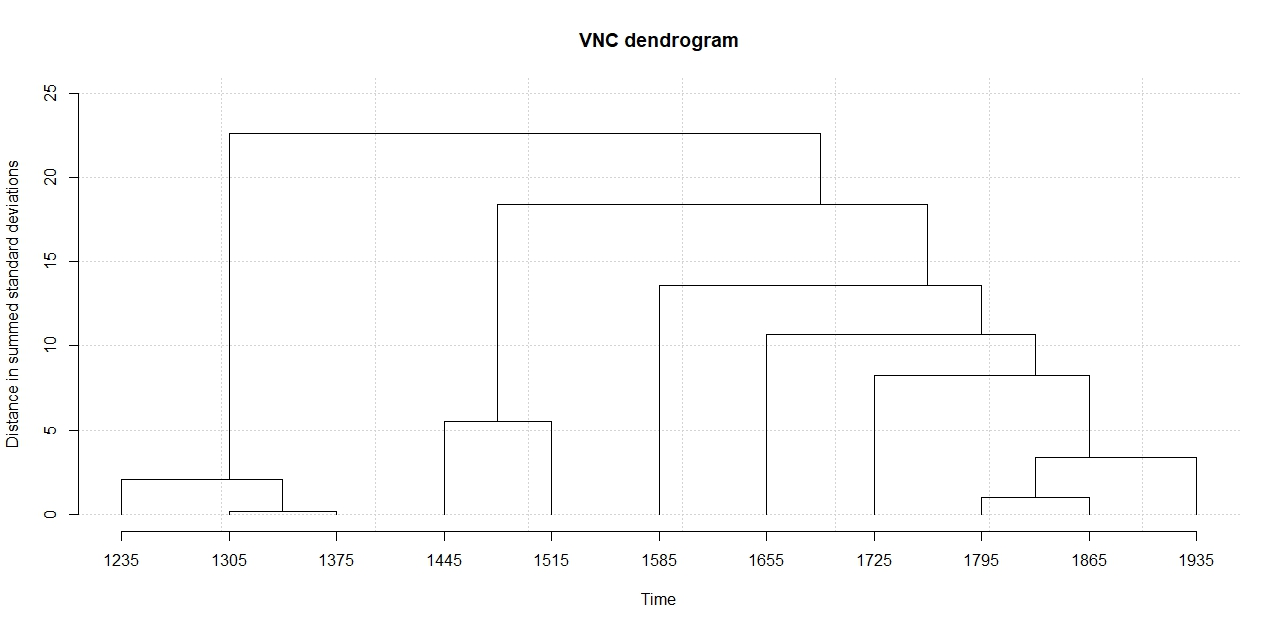
\includegraphics{ita_dendro_apr25.jpeg}
\caption{Dendogram Italian}
\end{figure}

\begin{figure}
\centering
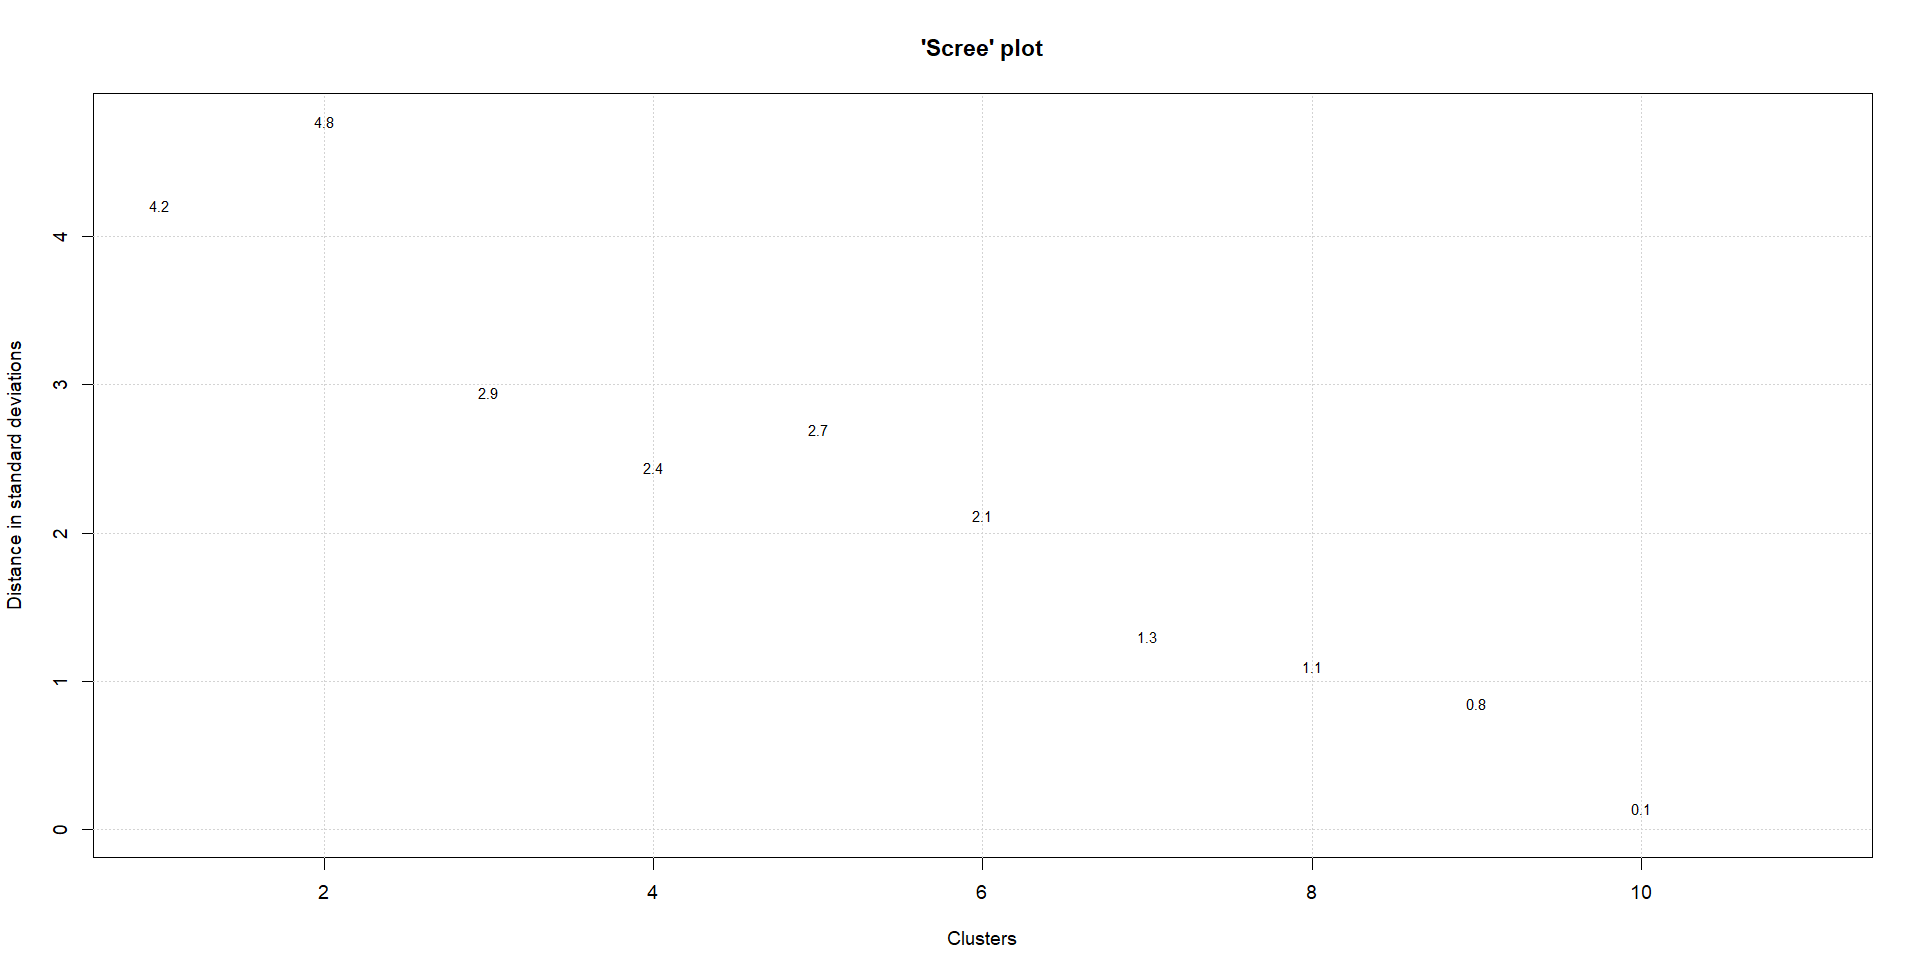
\includegraphics{ita_scree_apr25.jpeg}
\caption{Screeplot Italian}
\end{figure}

\begin{figure}
\centering
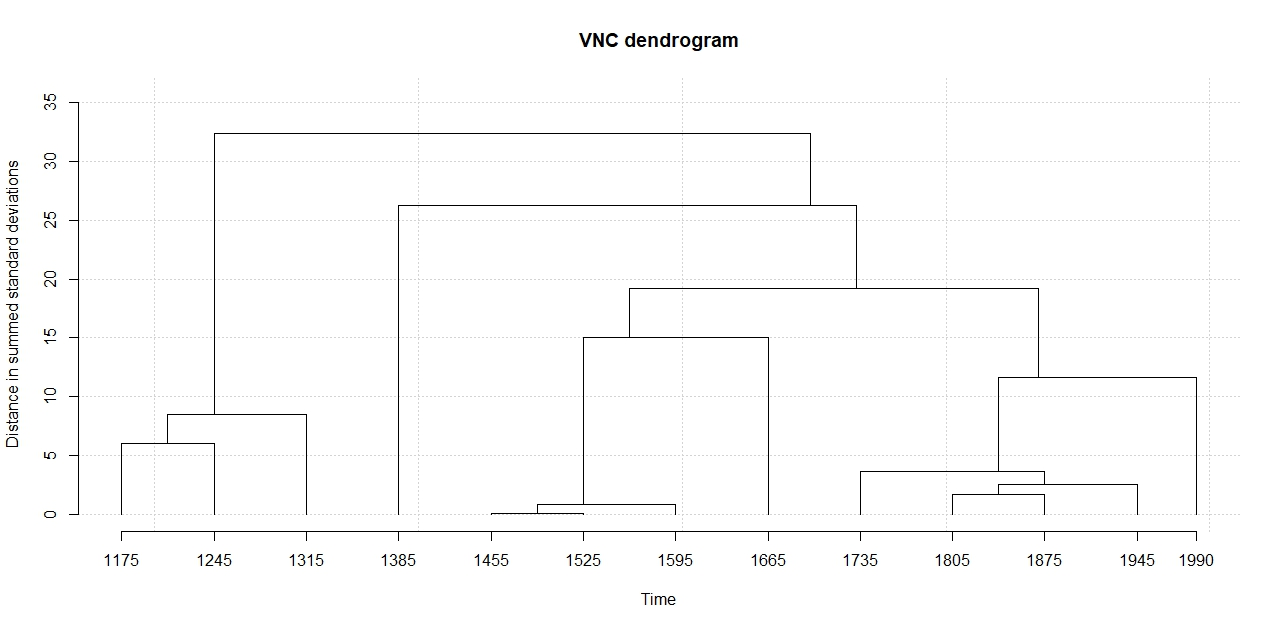
\includegraphics{es_dendro_apr25.jpeg}
\caption{Dendogram Spanish}
\end{figure}

\begin{figure}
\centering
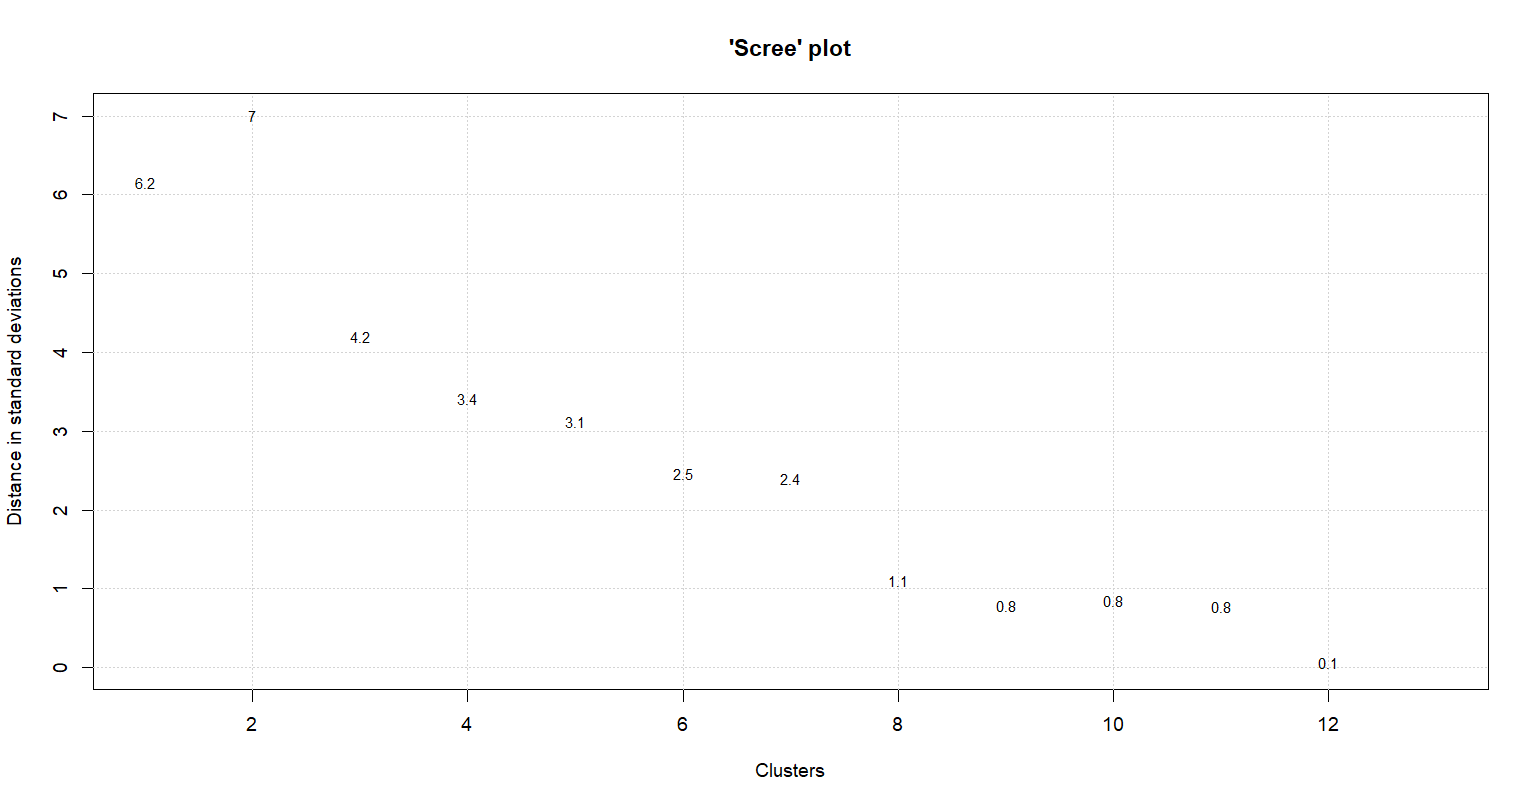
\includegraphics{es_scree_apr25.jpeg}
\caption{Screeplot Spanish}
\end{figure}

From the interpretation of the VNC results we end up with 4 significant
periods for the development of the causal vs.~non causal alternation in
Spanish, dividing our dataset in the following periods:
1140-1209,1210-1279, 1280-1559, 1560-2001. Data are distributed across
periods as summarised below. In Spanish causal uses are consistently
higher than noncausal ones, but always below 60\% except in the second
period where they reach 73\%.

\begin{Shaded}
\begin{Highlighting}[]
\NormalTok{esp}\OtherTok{\textless{}{-}}\NormalTok{esp }\SpecialCharTok{\%\textgreater{}\%} 
  \FunctionTok{mutate}\NormalTok{(}
    \AttributeTok{es\_vnc70\_apr25=}\FunctionTok{case\_when}\NormalTok{(}
\NormalTok{      year}\SpecialCharTok{\textless{}}\DecValTok{1350} \SpecialCharTok{\textasciitilde{}} \StringTok{"1140{-}1349"}\NormalTok{,}
\NormalTok{      year}\SpecialCharTok{\textless{}}\DecValTok{1420} \SpecialCharTok{\textasciitilde{}} \StringTok{"1350{-}1419"}\NormalTok{,}
\NormalTok{      year}\SpecialCharTok{\textless{}}\DecValTok{1700} \SpecialCharTok{\textasciitilde{}} \StringTok{"1420{-}1699"}\NormalTok{,}
\NormalTok{      year}\SpecialCharTok{\textless{}}\DecValTok{2002} \SpecialCharTok{\textasciitilde{}} \StringTok{"1700{-}2001"}
\NormalTok{    )}
\NormalTok{  )}

\NormalTok{summary\_es}\OtherTok{\textless{}{-}}\NormalTok{esp }\SpecialCharTok{\%\textgreater{}\%}
  \FunctionTok{group\_by}\NormalTok{ (es\_vnc70\_apr25, semantics) }\SpecialCharTok{\%\textgreater{}\%}
  \FunctionTok{summarise}\NormalTok{ (}\AttributeTok{n=}\FunctionTok{n}\NormalTok{()) }\SpecialCharTok{\%\textgreater{}\%}
  \FunctionTok{mutate}\NormalTok{(}\AttributeTok{rel.freq =} \FunctionTok{paste0}\NormalTok{(}\FunctionTok{round}\NormalTok{(}\DecValTok{100} \SpecialCharTok{*}\NormalTok{ n}\SpecialCharTok{/}\FunctionTok{sum}\NormalTok{(n), }\DecValTok{0}\NormalTok{), }\StringTok{"\%"}\NormalTok{))}

\NormalTok{summary\_es }\SpecialCharTok{\%\textgreater{}\%}  \FunctionTok{kbl}\NormalTok{(}\AttributeTok{booktabs =} \ConstantTok{TRUE}\NormalTok{, }\AttributeTok{col.names =} \FunctionTok{c}\NormalTok{(}\StringTok{"VNC periods"}\NormalTok{, }\StringTok{"Semantics"}\NormalTok{, }\StringTok{"Count"}\NormalTok{, }\StringTok{"Relative Frequency (\%)"}\NormalTok{), }\AttributeTok{caption =} \StringTok{"Spanish {-} Summary of the verb semantics by VNC periods"}\NormalTok{) }\SpecialCharTok{\%\textgreater{}\%}
   \FunctionTok{collapse\_rows}\NormalTok{(}\AttributeTok{column =} \DecValTok{1}\NormalTok{) }\SpecialCharTok{\%\textgreater{}\%} 
  \FunctionTok{kable\_styling}\NormalTok{() }
\end{Highlighting}
\end{Shaded}

\begin{table}
\centering
\caption{\label{tab:unnamed-chunk-7}Spanish - Summary of the verb semantics by VNC periods}
\centering
\begin{tabular}[t]{llrl}
\toprule
VNC periods & Semantics & Count & Relative Frequency (\%)\\
\midrule
 & caus & 434 & 55\%\\
\cmidrule{2-4}
\multirow{-2}{*}{\raggedright\arraybackslash 1140-1349} & noncaus & 348 & 45\%\\
\cmidrule{1-4}
 & caus & 92 & 73\%\\
\cmidrule{2-4}
\multirow{-2}{*}{\raggedright\arraybackslash 1350-1419} & noncaus & 34 & 27\%\\
\cmidrule{1-4}
 & caus & 1367 & 57\%\\
\cmidrule{2-4}
\multirow{-2}{*}{\raggedright\arraybackslash 1420-1699} & noncaus & 1044 & 43\%\\
\cmidrule{1-4}
 & caus & 1653 & 52\%\\
\cmidrule{2-4}
\multirow{-2}{*}{\raggedright\arraybackslash 1700-2001} & noncaus & 1523 & 48\%\\
\bottomrule
\end{tabular}
\end{table}

For Italian, the relevant 4 periods indicated by the dendogram are
1200-1409, 1410-1549, 1550-1619 and 1620-1968, Data are distributed
across periods as summarised below. In Italian, causal uses are
consistently more frequent than non causal ones, always higher than
60\%. Their relative frequency is at the highest in the second period,
when they reach 73\%, like in Spanish. However, the second VNC period in
Italian is about a century later than in Spanish.

\begin{Shaded}
\begin{Highlighting}[]
\NormalTok{ita}\OtherTok{\textless{}{-}}\NormalTok{ita }\SpecialCharTok{\%\textgreater{}\%} 
  \FunctionTok{mutate}\NormalTok{(}
    \AttributeTok{ita\_vnc70\_apr25=}\FunctionTok{case\_when}\NormalTok{(}
\NormalTok{      year}\SpecialCharTok{\textless{}}\DecValTok{1410} \SpecialCharTok{\textasciitilde{}} \StringTok{"1200{-}1409"}\NormalTok{,}
\NormalTok{      year}\SpecialCharTok{\textless{}}\DecValTok{1550} \SpecialCharTok{\textasciitilde{}} \StringTok{"1410{-}1549"}\NormalTok{,}
\NormalTok{      year}\SpecialCharTok{\textless{}}\DecValTok{1620} \SpecialCharTok{\textasciitilde{}} \StringTok{"1550{-}1619"}\NormalTok{,}
\NormalTok{      year}\SpecialCharTok{\textless{}=}\DecValTok{1970} \SpecialCharTok{\textasciitilde{}} \StringTok{"1620{-}1968"}
\NormalTok{    )}
\NormalTok{  )}

\NormalTok{summary\_ita}\OtherTok{\textless{}{-}}\NormalTok{ita }\SpecialCharTok{\%\textgreater{}\%}
  \FunctionTok{group\_by}\NormalTok{ (ita\_vnc70\_apr25, semantics) }\SpecialCharTok{\%\textgreater{}\%}
  \FunctionTok{summarise}\NormalTok{ (}\AttributeTok{n=}\FunctionTok{n}\NormalTok{()) }\SpecialCharTok{\%\textgreater{}\%}
  \FunctionTok{mutate}\NormalTok{(}\AttributeTok{rel.freq =} \FunctionTok{paste0}\NormalTok{(}\FunctionTok{round}\NormalTok{(}\DecValTok{100} \SpecialCharTok{*}\NormalTok{ n}\SpecialCharTok{/}\FunctionTok{sum}\NormalTok{(n), }\DecValTok{0}\NormalTok{), }\StringTok{"\%"}\NormalTok{))}

\NormalTok{summary\_ita }\SpecialCharTok{\%\textgreater{}\%}  \FunctionTok{kbl}\NormalTok{(}\AttributeTok{booktabs =} \ConstantTok{TRUE}\NormalTok{, }\AttributeTok{col.names =} \FunctionTok{c}\NormalTok{(}\StringTok{"VNC periods"}\NormalTok{, }\StringTok{"Semantics"}\NormalTok{, }\StringTok{"Count"}\NormalTok{, }\StringTok{"Relative Frequency (\%)"}\NormalTok{), }\AttributeTok{caption =} \StringTok{"Italian {-} Summary of the verb semantics by VNC periods"}\NormalTok{) }\SpecialCharTok{\%\textgreater{}\%}
   \FunctionTok{collapse\_rows}\NormalTok{(}\AttributeTok{column =} \DecValTok{1}\NormalTok{) }\SpecialCharTok{\%\textgreater{}\%} 
  \FunctionTok{kable\_styling}\NormalTok{() }
\end{Highlighting}
\end{Shaded}

\begin{table}
\centering
\caption{\label{tab:unnamed-chunk-8}Italian - Summary of the verb semantics by VNC periods}
\centering
\begin{tabular}[t]{llrl}
\toprule
VNC periods & Semantics & Count & Relative Frequency (\%)\\
\midrule
 & caus & 768 & 64\%\\
\cmidrule{2-4}
\multirow{-2}{*}{\raggedright\arraybackslash 1200-1409} & noncaus & 441 & 36\%\\
\cmidrule{1-4}
 & caus & 1135 & 73\%\\
\cmidrule{2-4}
\multirow{-2}{*}{\raggedright\arraybackslash 1410-1549} & noncaus & 421 & 27\%\\
\cmidrule{1-4}
 & caus & 695 & 67\%\\
\cmidrule{2-4}
\multirow{-2}{*}{\raggedright\arraybackslash 1550-1619} & noncaus & 335 & 33\%\\
\cmidrule{1-4}
 & caus & 2700 & 62\%\\
\cmidrule{2-4}
\multirow{-2}{*}{\raggedright\arraybackslash 1620-1968} & noncaus & 1635 & 38\%\\
\bottomrule
\end{tabular}
\end{table}

\subsubsection{\texorpdfstring{Calculate the
\texttt{Causalness\ Degree}}{Calculate the Causalness Degree}}\label{calculate-the-causalness-degree}

Once we found out the significant periods for the causal/non causal
alternation, we calculate the share of causal uses by verb lemma and by
period. Namely, every verb lemma in each of the four periods is assigned
a number between 0 and 1, indicating the proportion (\%) of causal uses
\emph{vs.} non causal uses. The table below summarises the distribution
of causal uses by lemma and period (variable \emph{caus\_use}).

Italian:

\begin{Shaded}
\begin{Highlighting}[]
\NormalTok{caus\_use\_ita}\OtherTok{\textless{}{-}}\NormalTok{ita }\SpecialCharTok{\%\textgreater{}\%}
  \FunctionTok{group\_by}\NormalTok{ (ita\_vnc70\_apr25, lemma, semantics) }\SpecialCharTok{\%\textgreater{}\%}
  \FunctionTok{summarise}\NormalTok{ (}\AttributeTok{n=}\FunctionTok{n}\NormalTok{()) }\SpecialCharTok{\%\textgreater{}\%}
  \FunctionTok{mutate}\NormalTok{(}\AttributeTok{caus\_use\_ita\_apr25 =}\NormalTok{ n}\SpecialCharTok{/}\FunctionTok{sum}\NormalTok{(n))}


\NormalTok{caus\_use\_ita}\OtherTok{\textless{}{-}}\NormalTok{caus\_use\_ita }\SpecialCharTok{\%\textgreater{}\%} \FunctionTok{filter}\NormalTok{(semantics}\SpecialCharTok{==}\StringTok{"caus"}\NormalTok{) }\SpecialCharTok{\%\textgreater{}\%} \FunctionTok{ungroup}\NormalTok{() }\SpecialCharTok{\%\textgreater{}\%} \FunctionTok{select}\NormalTok{ (}\SpecialCharTok{{-}}\NormalTok{semantics)}

\NormalTok{caus\_use\_ita }\SpecialCharTok{\%\textgreater{}\%}\NormalTok{ DT}\SpecialCharTok{::}\FunctionTok{datatable}\NormalTok{(}\AttributeTok{rownames=}\NormalTok{F, }\AttributeTok{filter=}\StringTok{"top"}\NormalTok{)}
\end{Highlighting}
\end{Shaded}

\includegraphics{Report_VNC_ita_es_publication_apr25_clean_files/figure-latex/unnamed-chunk-9-1.pdf}

Spanish:

\begin{Shaded}
\begin{Highlighting}[]
\NormalTok{caus\_use\_es }\OtherTok{\textless{}{-}}\NormalTok{esp }\SpecialCharTok{\%\textgreater{}\%}
  \FunctionTok{group\_by}\NormalTok{ (es\_vnc70\_apr25, lemma, semantics) }\SpecialCharTok{\%\textgreater{}\%}
  \FunctionTok{summarise}\NormalTok{ (}\AttributeTok{n=}\FunctionTok{n}\NormalTok{()) }\SpecialCharTok{\%\textgreater{}\%}
  \FunctionTok{mutate}\NormalTok{(}\AttributeTok{caus\_use\_es\_apr25 =}\NormalTok{ n}\SpecialCharTok{/}\FunctionTok{sum}\NormalTok{(n))}


\NormalTok{caus\_use\_es}\OtherTok{\textless{}{-}}\NormalTok{caus\_use\_es }\SpecialCharTok{\%\textgreater{}\%} \FunctionTok{filter}\NormalTok{(semantics}\SpecialCharTok{==}\StringTok{"caus"}\NormalTok{) }\SpecialCharTok{\%\textgreater{}\%} \FunctionTok{ungroup}\NormalTok{() }\SpecialCharTok{\%\textgreater{}\%} \FunctionTok{select}\NormalTok{ (}\SpecialCharTok{{-}}\NormalTok{semantics)}

\NormalTok{caus\_use\_es }\SpecialCharTok{\%\textgreater{}\%}\NormalTok{ DT}\SpecialCharTok{::}\FunctionTok{datatable}\NormalTok{(}\AttributeTok{rownames=}\NormalTok{F, }\AttributeTok{filter=}\StringTok{"top"}\NormalTok{)}
\end{Highlighting}
\end{Shaded}

\includegraphics{Report_VNC_ita_es_publication_apr25_clean_files/figure-latex/unnamed-chunk-10-1.pdf}

And finally rejoin the individual languages new information
(\texttt{period70,\ vnc\ and\ causalness\ degree}) to the main dataset:

\begin{Shaded}
\begin{Highlighting}[]
\FunctionTok{library}\NormalTok{(dplyr)}

\CommentTok{\# 1. Join caus\_use\_ita to ita by vnc and lemma}
\NormalTok{ita }\OtherTok{\textless{}{-}}\NormalTok{ ita }\SpecialCharTok{\%\textgreater{}\%}
  \FunctionTok{left\_join}\NormalTok{(caus\_use\_ita, }\AttributeTok{by =} \FunctionTok{c}\NormalTok{(}\StringTok{"ita\_vnc70\_apr25"} \OtherTok{=} \StringTok{"ita\_vnc70\_apr25"}\NormalTok{, }\StringTok{"lemma"} \OtherTok{=} \StringTok{"lemma"}\NormalTok{))}

\CommentTok{\# 2. Join caus\_use\_es to esp by vnc and lemma}
\NormalTok{esp }\OtherTok{\textless{}{-}}\NormalTok{ esp }\SpecialCharTok{\%\textgreater{}\%}
  \FunctionTok{left\_join}\NormalTok{(caus\_use\_es, }\AttributeTok{by =} \FunctionTok{c}\NormalTok{(}\StringTok{"es\_vnc70\_apr25"} \OtherTok{=} \StringTok{"es\_vnc70\_apr25"}\NormalTok{, }\StringTok{"lemma"} \OtherTok{=} \StringTok{"lemma"}\NormalTok{))}

\CommentTok{\# 3. Rename columns to match target names before merging into romall}
\NormalTok{ita }\OtherTok{\textless{}{-}}\NormalTok{ ita }\SpecialCharTok{\%\textgreater{}\%}
  \FunctionTok{rename}\NormalTok{(}
    \AttributeTok{vnc\_period\_apr25 =}\NormalTok{ ita\_vnc70\_apr25,}
    \AttributeTok{causalness\_degree\_apr25 =}\NormalTok{ caus\_use\_ita\_apr25}
\NormalTok{  )}

\NormalTok{esp }\OtherTok{\textless{}{-}}\NormalTok{ esp }\SpecialCharTok{\%\textgreater{}\%}
  \FunctionTok{rename}\NormalTok{(}
    \AttributeTok{vnc\_period\_apr25 =}\NormalTok{ es\_vnc70\_apr25,}
    \AttributeTok{causalness\_degree\_apr25 =}\NormalTok{ caus\_use\_es\_apr25}
\NormalTok{  )}

\CommentTok{\# 4. Bind the two enriched subsets together}
\NormalTok{combined }\OtherTok{\textless{}{-}} \FunctionTok{bind\_rows}\NormalTok{(ita, esp)}

\CommentTok{\# 5. Join back to romall by id and lemma}
\NormalTok{romall }\OtherTok{\textless{}{-}}\NormalTok{ romall }\SpecialCharTok{\%\textgreater{}\%}
  \FunctionTok{left\_join}\NormalTok{(combined }\SpecialCharTok{\%\textgreater{}\%} \FunctionTok{select}\NormalTok{(id, lemma, vnc\_period\_apr25, causalness\_degree\_apr25),}
            \AttributeTok{by =} \FunctionTok{c}\NormalTok{(}\StringTok{"id"}\NormalTok{, }\StringTok{"lemma"}\NormalTok{))}


\NormalTok{nc }\OtherTok{\textless{}{-}}\NormalTok{ nc }\SpecialCharTok{\%\textgreater{}\%}
  \FunctionTok{left\_join}\NormalTok{(combined }\SpecialCharTok{\%\textgreater{}\%} \FunctionTok{select}\NormalTok{(id, lemma, vnc\_period\_apr25, causalness\_degree\_apr25),}
            \AttributeTok{by =} \FunctionTok{c}\NormalTok{(}\StringTok{"id"}\NormalTok{, }\StringTok{"lemma"}\NormalTok{))}
\end{Highlighting}
\end{Shaded}

\begin{Shaded}
\begin{Highlighting}[]
\CommentTok{\#only run this if you want to save the results of the VNC in a new xlsx file}

\NormalTok{openxlsx}\SpecialCharTok{::}\FunctionTok{write.xlsx}\NormalTok{(romall, }\StringTok{"romall\_new\_VNC.xlsx"}\NormalTok{)}
\NormalTok{openxlsx}\SpecialCharTok{::}\FunctionTok{write.xlsx}\NormalTok{(nc, }\StringTok{"noncaus\_new\_VNC.xlsx"}\NormalTok{)}
\end{Highlighting}
\end{Shaded}

\section{Part II: Frequency effects of causal degree on anticausative
marking over
time}\label{part-ii-frequency-effects-of-causal-degree-on-anticausative-marking-over-time}

\begin{Shaded}
\begin{Highlighting}[]
\CommentTok{\# only non causal, verbs with categorical selection removed}

\NormalTok{ita\_nc}\OtherTok{\textless{}{-}}\NormalTok{nc }\SpecialCharTok{\%\textgreater{}\%} \FunctionTok{filter}\NormalTok{(language}\SpecialCharTok{==}\StringTok{"italian"}\NormalTok{)}
\NormalTok{es\_nc}\OtherTok{\textless{}{-}}\NormalTok{nc }\SpecialCharTok{\%\textgreater{}\%} \FunctionTok{filter}\NormalTok{(language}\SpecialCharTok{==}\StringTok{"spanish"}\NormalTok{)}



\NormalTok{ita\_nc}\OtherTok{\textless{}{-}}\NormalTok{ita\_nc }\SpecialCharTok{\%\textgreater{}\%} \FunctionTok{select}\NormalTok{(id, coding, meaning, lemma, vnc\_period\_apr25, causalness\_degree\_apr25)}

\NormalTok{ita\_nc}\OtherTok{\textless{}{-}}\NormalTok{ita\_nc }\SpecialCharTok{\%\textgreater{}\%} \FunctionTok{rename}\NormalTok{(}\AttributeTok{period=}\NormalTok{vnc\_period\_apr25, }\AttributeTok{causalness\_degree=}\NormalTok{causalness\_degree\_apr25)}

\NormalTok{es\_nc}\OtherTok{\textless{}{-}}\NormalTok{es\_nc }\SpecialCharTok{\%\textgreater{}\%} \FunctionTok{select}\NormalTok{(id, coding, meaning, lemma, vnc\_period\_apr25, causalness\_degree\_apr25)}

\NormalTok{es\_nc}\OtherTok{\textless{}{-}}\NormalTok{es\_nc }\SpecialCharTok{\%\textgreater{}\%} \FunctionTok{rename}\NormalTok{(}\AttributeTok{period=}\NormalTok{vnc\_period\_apr25, }\AttributeTok{causalness\_degree=}\NormalTok{causalness\_degree\_apr25)}
\end{Highlighting}
\end{Shaded}

\subsection{Italian data: prepare for Beta
Regression}\label{italian-data-prepare-for-beta-regression}

Subset the Italian data to obtain unique combinations of lemma and
period.

\begin{itemize}
\tightlist
\item
  Step 1: Aggregate data to calculate the proportion of anticausative
  codings
\end{itemize}

\begin{Shaded}
\begin{Highlighting}[]
\NormalTok{ita\_agg }\OtherTok{\textless{}{-}}\NormalTok{ ita\_nc }\SpecialCharTok{\%\textgreater{}\%}
  \FunctionTok{group\_by}\NormalTok{(lemma, period) }\SpecialCharTok{\%\textgreater{}\%}
  \FunctionTok{summarise}\NormalTok{(}
    \AttributeTok{anticausative\_count =} \FunctionTok{sum}\NormalTok{(coding }\SpecialCharTok{==} \StringTok{"antic"}\NormalTok{),}
    \AttributeTok{total\_count =} \FunctionTok{n}\NormalTok{(),}
    \AttributeTok{proportion\_anticausative =}\NormalTok{ anticausative\_count }\SpecialCharTok{/}\NormalTok{ total\_count,}
    \AttributeTok{causalness\_degree =} \FunctionTok{first}\NormalTok{(causalness\_degree),}
\NormalTok{      ) }\SpecialCharTok{\%\textgreater{}\%}
  \FunctionTok{ungroup}\NormalTok{()}
\end{Highlighting}
\end{Shaded}

\begin{itemize}
\tightlist
\item
  Step 2: Create a lagged causalness\_degree variable
\end{itemize}

\begin{Shaded}
\begin{Highlighting}[]
\NormalTok{ita\_agg }\OtherTok{\textless{}{-}}\NormalTok{ ita\_agg }\SpecialCharTok{\%\textgreater{}\%}
  \FunctionTok{arrange}\NormalTok{(lemma, period) }\SpecialCharTok{\%\textgreater{}\%}
  \FunctionTok{group\_by}\NormalTok{(lemma) }\SpecialCharTok{\%\textgreater{}\%}
  \FunctionTok{mutate}\NormalTok{(}\AttributeTok{causalness\_lagged =} \FunctionTok{lag}\NormalTok{(causalness\_degree)) }\SpecialCharTok{\%\textgreater{}\%}
  \FunctionTok{ungroup}\NormalTok{() }\SpecialCharTok{\%\textgreater{}\%}
  \CommentTok{\# Remove rows without previous causalness\_degree (period 1)}
  \FunctionTok{filter}\NormalTok{(}\SpecialCharTok{!}\FunctionTok{is.na}\NormalTok{(causalness\_lagged))}
\end{Highlighting}
\end{Shaded}

\begin{itemize}
\tightlist
\item
  Step 3: Adjust proportions slightly to avoid exact 0 and 1
\end{itemize}

\begin{Shaded}
\begin{Highlighting}[]
\NormalTok{ita\_agg }\OtherTok{\textless{}{-}}\NormalTok{ ita\_agg }\SpecialCharTok{\%\textgreater{}\%}
  \FunctionTok{mutate}\NormalTok{(}\AttributeTok{proportion\_adj =}\NormalTok{ (proportion\_anticausative }\SpecialCharTok{*}\NormalTok{ (total\_count }\SpecialCharTok{{-}} \DecValTok{1}\NormalTok{) }\SpecialCharTok{+} \FloatTok{0.5}\NormalTok{) }\SpecialCharTok{/}\NormalTok{ total\_count)}

\NormalTok{ita\_agg}\OtherTok{\textless{}{-}}\NormalTok{ita\_agg }\SpecialCharTok{\%\textgreater{}\%}
  \FunctionTok{filter}\NormalTok{(}\SpecialCharTok{!}\FunctionTok{is.na}\NormalTok{(proportion\_adj), }\SpecialCharTok{!}\FunctionTok{is.na}\NormalTok{(causalness\_lagged))}

\NormalTok{ita\_agg }\OtherTok{\textless{}{-}}\NormalTok{ ita\_agg }\SpecialCharTok{\%\textgreater{}\%}
  \FunctionTok{mutate}\NormalTok{(}\FunctionTok{across}\NormalTok{(}\DecValTok{5}\SpecialCharTok{:}\DecValTok{8}\NormalTok{, }\SpecialCharTok{\textasciitilde{}} \FunctionTok{round}\NormalTok{(.x, }\DecValTok{2}\NormalTok{))) }
\end{Highlighting}
\end{Shaded}

\subsection{Spanish data: prepare for Beta
Regression}\label{spanish-data-prepare-for-beta-regression}

Subset the Spanish data to obtain unique combinations of lemma and
period.

\begin{itemize}
\tightlist
\item
  Step 1: Aggregate data to calculate the proportion of anticausative
  codings:
\end{itemize}

\begin{Shaded}
\begin{Highlighting}[]
\NormalTok{es\_agg }\OtherTok{\textless{}{-}}\NormalTok{ es\_nc }\SpecialCharTok{\%\textgreater{}\%}
  \FunctionTok{group\_by}\NormalTok{(lemma, period) }\SpecialCharTok{\%\textgreater{}\%}
  \FunctionTok{summarise}\NormalTok{(}
    \AttributeTok{anticausative\_count =} \FunctionTok{sum}\NormalTok{(coding }\SpecialCharTok{==} \StringTok{"antic"}\NormalTok{),}
    \AttributeTok{total\_count =} \FunctionTok{n}\NormalTok{(),}
    \AttributeTok{proportion\_anticausative =}\NormalTok{ anticausative\_count }\SpecialCharTok{/}\NormalTok{ total\_count,}
    \AttributeTok{causalness\_degree =} \FunctionTok{first}\NormalTok{(causalness\_degree),}
\NormalTok{    ) }\SpecialCharTok{\%\textgreater{}\%}
  \FunctionTok{ungroup}\NormalTok{()}
\end{Highlighting}
\end{Shaded}

\begin{itemize}
\tightlist
\item
  Step 2: Create a lagged causalness\_degree variable:
\end{itemize}

\begin{Shaded}
\begin{Highlighting}[]
\NormalTok{es\_agg }\OtherTok{\textless{}{-}}\NormalTok{ es\_agg }\SpecialCharTok{\%\textgreater{}\%}
  \FunctionTok{arrange}\NormalTok{(lemma, period) }\SpecialCharTok{\%\textgreater{}\%}
  \FunctionTok{group\_by}\NormalTok{(lemma) }\SpecialCharTok{\%\textgreater{}\%}
  \FunctionTok{mutate}\NormalTok{(}\AttributeTok{causalness\_lagged =} \FunctionTok{lag}\NormalTok{(causalness\_degree)) }\SpecialCharTok{\%\textgreater{}\%}
  \FunctionTok{ungroup}\NormalTok{() }\SpecialCharTok{\%\textgreater{}\%}
  \CommentTok{\# Remove rows without previous causalness\_degree (period 1)}
  \FunctionTok{filter}\NormalTok{(}\SpecialCharTok{!}\FunctionTok{is.na}\NormalTok{(causalness\_lagged)) }
\end{Highlighting}
\end{Shaded}

\begin{itemize}
\tightlist
\item
  Step 3:Adjust proportions slightly to avoid exact 0 and 1
\end{itemize}

\begin{Shaded}
\begin{Highlighting}[]
\NormalTok{es\_agg }\OtherTok{\textless{}{-}}\NormalTok{ es\_agg }\SpecialCharTok{\%\textgreater{}\%}
  \FunctionTok{mutate}\NormalTok{(}\AttributeTok{proportion\_adj =}\NormalTok{ (proportion\_anticausative }\SpecialCharTok{*}\NormalTok{ (total\_count }\SpecialCharTok{{-}} \DecValTok{1}\NormalTok{) }\SpecialCharTok{+} \FloatTok{0.5}\NormalTok{) }\SpecialCharTok{/}\NormalTok{ total\_count)}

\NormalTok{es\_agg}\OtherTok{\textless{}{-}}\NormalTok{es\_agg }\SpecialCharTok{\%\textgreater{}\%}
  \FunctionTok{filter}\NormalTok{(}\SpecialCharTok{!}\FunctionTok{is.na}\NormalTok{(proportion\_adj), }\SpecialCharTok{!}\FunctionTok{is.na}\NormalTok{(causalness\_lagged))}

\NormalTok{es\_agg }\OtherTok{\textless{}{-}}\NormalTok{ es\_agg }\SpecialCharTok{\%\textgreater{}\%}
  \FunctionTok{mutate}\NormalTok{(}\FunctionTok{across}\NormalTok{(}\DecValTok{5}\SpecialCharTok{:}\DecValTok{8}\NormalTok{, }\SpecialCharTok{\textasciitilde{}} \FunctionTok{round}\NormalTok{(.x, }\DecValTok{2}\NormalTok{))) }
\end{Highlighting}
\end{Shaded}

\subsection{Fit the Beta Regression
model}\label{fit-the-beta-regression-model}

\begin{itemize}
\tightlist
\item
  Step 1: join the Italian and Spanish sub-dataset
\item
  Step 2: make the categorical variable into factors; transform
  \texttt{period} into a numeric variable to be able to use it as a
  smooth term
\end{itemize}

\begin{Shaded}
\begin{Highlighting}[]
\CommentTok{\# Step 1}
\DocumentationTok{\#\# Add a column to each dataset to distinguish them}
\NormalTok{italian }\OtherTok{\textless{}{-}}\NormalTok{ ita\_agg }\SpecialCharTok{\%\textgreater{}\%}
  \FunctionTok{mutate}\NormalTok{(}\AttributeTok{language =} \StringTok{"Italian"}\NormalTok{)}

\NormalTok{spanish }\OtherTok{\textless{}{-}}\NormalTok{ es\_agg }\SpecialCharTok{\%\textgreater{}\%}
  \FunctionTok{mutate}\NormalTok{(}\AttributeTok{language =} \StringTok{"Spanish"}\NormalTok{)}

\DocumentationTok{\#\# Combine the datasets using bind\_rows()}
\NormalTok{join }\OtherTok{\textless{}{-}} \FunctionTok{bind\_rows}\NormalTok{(italian, spanish)}

\DocumentationTok{\#\# View the combined dataset}
\FunctionTok{head}\NormalTok{(join)}
\end{Highlighting}
\end{Shaded}

\begin{verbatim}
## # A tibble: 6 x 9
##   lemma     period    anticausative_count total_count proportion_anticausative
##   <chr>     <chr>                   <int>       <int>                    <dbl>
## 1 affondare 1410-1549                   0           1                     0   
## 2 affondare 1550-1619                   1           2                     0.5 
## 3 affondare 1620-1968                   5          21                     0.24
## 4 alzare    1410-1549                  14          16                     0.88
## 5 alzare    1550-1619                  32          32                     1   
## 6 alzare    1620-1968                 155         155                     1   
## # i 4 more variables: causalness_degree <dbl>, causalness_lagged <dbl>,
## #   proportion_adj <dbl>, language <chr>
\end{verbatim}

\begin{Shaded}
\begin{Highlighting}[]
\CommentTok{\# Step 2: prepare factors variables}

\NormalTok{join}\SpecialCharTok{$}\NormalTok{language}\OtherTok{\textless{}{-}}\FunctionTok{as.factor}\NormalTok{(join}\SpecialCharTok{$}\NormalTok{language)}
\NormalTok{join}\SpecialCharTok{$}\NormalTok{period\_cat}\OtherTok{\textless{}{-}}\FunctionTok{as.factor}\NormalTok{(join}\SpecialCharTok{$}\NormalTok{period)}
\NormalTok{join}\SpecialCharTok{$}\NormalTok{period}\OtherTok{\textless{}{-}}\FunctionTok{as.factor}\NormalTok{(join}\SpecialCharTok{$}\NormalTok{period)}

\NormalTok{join}\SpecialCharTok{$}\NormalTok{period }\OtherTok{\textless{}{-}} \FunctionTok{as.numeric}\NormalTok{(join}\SpecialCharTok{$}\NormalTok{period\_cat)}
\end{Highlighting}
\end{Shaded}

\begin{itemize}
\item
  Step 3: Fit a beta regression model with \texttt{mgvc::gam}:
  \emph{model1} is the maximal model which includes
\item
  \texttt{language} as a main effect; You must include \texttt{language}
  as a main effect in the model if it is a factor, when you use it as a
  smooth modifier (see argument by= below)
\item
  \texttt{s(causalness\_lagged,\ k=20)} and \texttt{s(period,\ k=5)},
  global smooth terms
\item
  \texttt{s(causalness\_lagged,\ by\ =\ language,\ k\ =\ 20,\ bs\ =\ "cs",\ m\ =\ 1)}
  and
  \texttt{s(period,\ by\ =\ language,\ k\ =\ 5,\ bs\ =\ "cs",\ m=\ 1)}
  as group-wise smooths (by \texttt{language})
\item
  \texttt{family\ =\ betar(...)}: This tells the model to use a beta
  regression family, which is designed for modeling proportions or rates
  --- i.e., values that are strictly between 0 and 1 (like 0.23 or
  0.85).
\item
  \texttt{link\ =\ "logit"}:this defines the link function, which
  transforms the predicted values to stay within the (0, 1) range.
\end{itemize}

\begin{Shaded}
\begin{Highlighting}[]
\NormalTok{model1 }\OtherTok{\textless{}{-}} \FunctionTok{gam}\NormalTok{(}
\NormalTok{  proportion\_anticausative }\SpecialCharTok{\textasciitilde{}} 
\NormalTok{    language }\SpecialCharTok{+} \CommentTok{\#you must include interaction terms as main effects too!}
    \FunctionTok{s}\NormalTok{(causalness\_lagged, }\AttributeTok{k=}\DecValTok{20}\NormalTok{)}\SpecialCharTok{+}
    \FunctionTok{s}\NormalTok{(period, }\AttributeTok{k=}\DecValTok{5}\NormalTok{)}\SpecialCharTok{+}
    \FunctionTok{s}\NormalTok{(causalness\_lagged, }\AttributeTok{by =}\NormalTok{ language, }\AttributeTok{k =} \DecValTok{20}\NormalTok{, }\AttributeTok{bs =} \StringTok{"cs"}\NormalTok{, }\AttributeTok{m =} \DecValTok{1}\NormalTok{) }\SpecialCharTok{+} 
    \FunctionTok{s}\NormalTok{(period, }\AttributeTok{by =}\NormalTok{ language, }\AttributeTok{k =} \DecValTok{5}\NormalTok{, }\AttributeTok{bs =} \StringTok{"cs"}\NormalTok{, }\AttributeTok{m=} \DecValTok{1}\NormalTok{),   }
  \AttributeTok{family =} \FunctionTok{betar}\NormalTok{(}\AttributeTok{link =} \StringTok{"logit"}\NormalTok{),                 }
  \AttributeTok{data =}\NormalTok{ join}
\NormalTok{)}

\CommentTok{\# Summarize the model}
\FunctionTok{summary}\NormalTok{(model1)}
\end{Highlighting}
\end{Shaded}

\begin{verbatim}
## 
## Family: Beta regression(0.253) 
## Link function: logit 
## 
## Formula:
## proportion_anticausative ~ language + s(causalness_lagged, k = 20) + 
##     s(period, k = 5) + s(causalness_lagged, by = language, k = 20, 
##     bs = "cs", m = 1) + s(period, by = language, k = 5, bs = "cs", 
##     m = 1)
## 
## Parametric coefficients:
##                 Estimate Std. Error z value Pr(>|z|)    
## (Intercept)       0.6836     0.1771   3.859 0.000114 ***
## languageSpanish   0.1966     0.2683   0.733 0.463758    
## ---
## Signif. codes:  0 '***' 0.001 '**' 0.01 '*' 0.05 '.' 0.1 ' ' 1
## 
## Approximate significance of smooth terms:
##                                            edf Ref.df Chi.sq  p-value    
## s(causalness_lagged)                 1.000e+00  1.000 13.596 0.000227 ***
## s(period)                            1.027e+00  1.052  1.763 0.201614    
## s(causalness_lagged):languageItalian 5.368e-03 19.000  0.005 0.059742 .  
## s(causalness_lagged):languageSpanish 9.067e-01 19.000  4.093 0.023175 *  
## s(period):languageItalian            8.323e-05  2.000  0.000 0.680123    
## s(period):languageSpanish            9.553e-05  2.000  0.000 0.622924    
## ---
## Signif. codes:  0 '***' 0.001 '**' 0.01 '*' 0.05 '.' 0.1 ' ' 1
## 
## R-sq.(adj) =  0.102   Deviance explained = -1.4%
## -REML = -828.02  Scale est. = 1         n = 99
\end{verbatim}

\begin{Shaded}
\begin{Highlighting}[]
\FunctionTok{gam.check}\NormalTok{(model1)}
\end{Highlighting}
\end{Shaded}

\includegraphics{Report_VNC_ita_es_publication_apr25_clean_files/figure-latex/unnamed-chunk-22-1.pdf}

\begin{verbatim}
## 
## Method: REML   Optimizer: outer newton
## full convergence after 11 iterations.
## Gradient range [-0.0007619733,1.953451e-05]
## (score -828.022 & scale 1).
## Hessian positive definite, eigenvalue range [2.678687e-05,68.58312].
## Model rank =  71 / 71
\end{verbatim}

\begin{verbatim}
## Basis dimension (k) checking results. Low p-value (k-index<1) may
## indicate that k is too low, especially if edf is close to k'.
## 
##                                            k'      edf k-index p-value
## s(causalness_lagged)                 1.90e+01 1.00e+00    1.00    0.46
## s(period)                            4.00e+00 1.03e+00    1.05    0.69
## s(causalness_lagged):languageItalian 1.90e+01 5.37e-03    1.00    0.54
## s(causalness_lagged):languageSpanish 1.90e+01 9.07e-01    1.00    0.52
## s(period):languageItalian            4.00e+00 8.32e-05    1.05    0.68
## s(period):languageSpanish            4.00e+00 9.55e-05    1.05    0.68
\end{verbatim}

The function \texttt{gam.check()} runs a set of diagnostic checks on
your fitted gam model (like model1). It's used to evaluate whether your
model is well-specified and whether the smoothing basis (the k values)
is adequate. * k-index -- Should ideally be ≥ 1; * values \textless{} 1
may mean k is too low. p-value -- If this is low (e.g.~\textless{} 0.05)
and edf ≈ k', you may need a larger k.

Here all p-values are high and edf is well below k', so our smooth terms
are well-behaved and the choice of k is appropriate.

However, the summary indicates that the \texttt{period} smooth and its
group-wise interaction are non-significant. We proceed with a backward
selection.

\begin{itemize}
\tightlist
\item
  Step 3: Backward selection
\end{itemize}

In \emph{model2} we start by removing
\texttt{s(period,\ by\ =\ language,\ k\ =\ 5,\ bs\ =\ "cs",\ m=\ 1)}. We
check the difference with three different methods: +
\texttt{compareML()} (from the itsadug package) compares two or more gam
or gamm models using AIC, BIC, log-likelihood, and explained deviance. +
\texttt{anova.gam()} compares two nested GAM models (e.g., model1 and a
simpler model2) using a likelihood ratio test (Chi-squared test) +
\texttt{AIC()}: it calculates the AIC of the two models, which is a
measure of model fit that balances goodness-of-fit with model complexity
(penalizes overfitting)

These three tests tell us that although AIC of model1 is better (also
shown by the ANOVA), model2 is preferred.

So we take \emph{model2} to be better, and we proceed looking at its
summary which shows that \texttt{s(period)} is non-significant. We fit
\emph{model3} without it, and use the same tests. All of them show that
\emph{model3} is better.

We proceed by removing \texttt{s(causalness\_lagged,\ k=20)}
(non-signitcant in \emph{model3}) in \emph{model4}, and all the tests
indicate that this is the best fitted model (see also the
\texttt{gam.check} output).

\begin{Shaded}
\begin{Highlighting}[]
\CommentTok{\#remove s(period, by = language, k = 5, bs = "cs", m= 1),   }

\NormalTok{model2 }\OtherTok{\textless{}{-}} \FunctionTok{gam}\NormalTok{(}
\NormalTok{  proportion\_anticausative }\SpecialCharTok{\textasciitilde{}} 
\NormalTok{    language }\SpecialCharTok{+} 
    \FunctionTok{s}\NormalTok{(causalness\_lagged, }\AttributeTok{k=}\DecValTok{20}\NormalTok{)}\SpecialCharTok{+}
    \FunctionTok{s}\NormalTok{(period, }\AttributeTok{k=}\DecValTok{5}\NormalTok{)}\SpecialCharTok{+}
    \FunctionTok{s}\NormalTok{(causalness\_lagged, }\AttributeTok{by =}\NormalTok{ language, }\AttributeTok{k =} \DecValTok{20}\NormalTok{, }\AttributeTok{bs =} \StringTok{"cs"}\NormalTok{, }\AttributeTok{m =} \DecValTok{1}\NormalTok{),}
  \AttributeTok{family =} \FunctionTok{betar}\NormalTok{(}\AttributeTok{link =} \StringTok{"logit"}\NormalTok{),                 }
  \AttributeTok{data =}\NormalTok{ join}
\NormalTok{)}

\FunctionTok{anova.gam}\NormalTok{(model1, model2, }\AttributeTok{test =} \StringTok{"Chisq"}\NormalTok{) }
\end{Highlighting}
\end{Shaded}

\begin{verbatim}
## Analysis of Deviance Table
## 
## Model 1: proportion_anticausative ~ language + s(causalness_lagged, k = 20) + 
##     s(period, k = 5) + s(causalness_lagged, by = language, k = 20, 
##     bs = "cs", m = 1) + s(period, by = language, k = 5, bs = "cs", 
##     m = 1)
## Model 2: proportion_anticausative ~ language + s(causalness_lagged, k = 20) + 
##     s(period, k = 5) + s(causalness_lagged, by = language, k = 20, 
##     bs = "cs", m = 1)
##   Resid. Df Resid. Dev       Df Deviance Pr(>Chi)  
## 1    93.449    -1666.3                             
## 2    93.435    -1666.3 0.014374 0.010322  0.03322 *
## ---
## Signif. codes:  0 '***' 0.001 '**' 0.01 '*' 0.05 '.' 0.1 ' ' 1
\end{verbatim}

\begin{Shaded}
\begin{Highlighting}[]
\FunctionTok{compareML}\NormalTok{(model1, model2)}
\end{Highlighting}
\end{Shaded}

\begin{verbatim}
## model1: proportion_anticausative ~ language + s(causalness_lagged, k = 20) + 
##     s(period, k = 5) + s(causalness_lagged, by = language, k = 20, 
##     bs = "cs", m = 1) + s(period, by = language, k = 5, bs = "cs", 
##     m = 1)
## 
## model2: proportion_anticausative ~ language + s(causalness_lagged, k = 20) + 
##     s(period, k = 5) + s(causalness_lagged, by = language, k = 20, 
##     bs = "cs", m = 1)
## 
## Model model2 preferred: lower REML score (0.000), and lower df (2.000).
## -----
##    Model    Score Edf Difference    Df
## 1 model1 -828.022  10                 
## 2 model2 -828.022   8     -0.000 2.000
## 
## AIC difference: -0.01, model model1 has lower AIC.
\end{verbatim}

\begin{Shaded}
\begin{Highlighting}[]
\FunctionTok{AIC}\NormalTok{(model1, model2)}
\end{Highlighting}
\end{Shaded}

\begin{verbatim}
##              df       AIC
## model1 6.244764 -1653.798
## model2 6.254698 -1653.788
\end{verbatim}

\begin{Shaded}
\begin{Highlighting}[]
\FunctionTok{summary}\NormalTok{(model2)}
\end{Highlighting}
\end{Shaded}

\begin{verbatim}
## 
## Family: Beta regression(0.253) 
## Link function: logit 
## 
## Formula:
## proportion_anticausative ~ language + s(causalness_lagged, k = 20) + 
##     s(period, k = 5) + s(causalness_lagged, by = language, k = 20, 
##     bs = "cs", m = 1)
## 
## Parametric coefficients:
##                 Estimate Std. Error z value Pr(>|z|)    
## (Intercept)       0.6837     0.1772   3.859 0.000114 ***
## languageSpanish   0.1960     0.2685   0.730 0.465291    
## ---
## Signif. codes:  0 '***' 0.001 '**' 0.01 '*' 0.05 '.' 0.1 ' ' 1
## 
## Approximate significance of smooth terms:
##                                          edf Ref.df Chi.sq  p-value    
## s(causalness_lagged)                 1.00017  1.000 13.053 0.000303 ***
## s(period)                            1.03086  1.061  1.773 0.203199    
## s(causalness_lagged):languageItalian 0.01013 19.000  0.010 0.059782 .  
## s(causalness_lagged):languageSpanish 0.90324 19.000  4.006 0.023209 *  
## ---
## Signif. codes:  0 '***' 0.001 '**' 0.01 '*' 0.05 '.' 0.1 ' ' 1
## 
## R-sq.(adj) =  0.102   Deviance explained = -1.4%
## -REML = -828.02  Scale est. = 1         n = 99
\end{verbatim}

\begin{Shaded}
\begin{Highlighting}[]
\CommentTok{\# remove \#s(period, k=5)}
\NormalTok{model3 }\OtherTok{\textless{}{-}} \FunctionTok{gam}\NormalTok{(}
\NormalTok{  proportion\_anticausative }\SpecialCharTok{\textasciitilde{}} 
\NormalTok{    language }\SpecialCharTok{+}
    \FunctionTok{s}\NormalTok{(causalness\_lagged, }\AttributeTok{k=}\DecValTok{20}\NormalTok{)}\SpecialCharTok{+}
    \FunctionTok{s}\NormalTok{(causalness\_lagged, }\AttributeTok{by =}\NormalTok{ language, }\AttributeTok{k =} \DecValTok{20}\NormalTok{, }\AttributeTok{bs =} \StringTok{"cs"}\NormalTok{, }\AttributeTok{m =} \DecValTok{1}\NormalTok{),}
  \AttributeTok{family =} \FunctionTok{betar}\NormalTok{(}\AttributeTok{link =} \StringTok{"logit"}\NormalTok{),                 }
  \AttributeTok{data =}\NormalTok{ join}
\NormalTok{)}

\FunctionTok{summary}\NormalTok{(model3)}
\end{Highlighting}
\end{Shaded}

\begin{verbatim}
## 
## Family: Beta regression(0.25) 
## Link function: logit 
## 
## Formula:
## proportion_anticausative ~ language + s(causalness_lagged, k = 20) + 
##     s(causalness_lagged, by = language, k = 20, bs = "cs", m = 1)
## 
## Parametric coefficients:
##                 Estimate Std. Error z value Pr(>|z|)    
## (Intercept)       0.6826     0.1767   3.862 0.000112 ***
## languageSpanish   0.2038     0.2671   0.763 0.445554    
## ---
## Signif. codes:  0 '***' 0.001 '**' 0.01 '*' 0.05 '.' 0.1 ' ' 1
## 
## Approximate significance of smooth terms:
##                                          edf Ref.df Chi.sq p-value  
## s(causalness_lagged)                 1.00055  1.001  0.856  0.3551  
## s(causalness_lagged):languageItalian 0.91942 19.000  3.426  0.0258 *
## s(causalness_lagged):languageSpanish 0.03915 19.000  0.039  0.0452 *
## ---
## Signif. codes:  0 '***' 0.001 '**' 0.01 '*' 0.05 '.' 0.1 ' ' 1
## 
## R-sq.(adj) =  0.117   Deviance explained = -1.24%
## -REML = -828.3  Scale est. = 1         n = 99
\end{verbatim}

\begin{Shaded}
\begin{Highlighting}[]
\FunctionTok{anova.gam}\NormalTok{(model3, model2, }\AttributeTok{test =} \StringTok{"Chisq"}\NormalTok{) }
\end{Highlighting}
\end{Shaded}

\begin{verbatim}
## Analysis of Deviance Table
## 
## Model 1: proportion_anticausative ~ language + s(causalness_lagged, k = 20) + 
##     s(causalness_lagged, by = language, k = 20, bs = "cs", m = 1)
## Model 2: proportion_anticausative ~ language + s(causalness_lagged, k = 20) + 
##     s(period, k = 5) + s(causalness_lagged, by = language, k = 20, 
##     bs = "cs", m = 1)
##   Resid. Df Resid. Dev      Df Deviance Pr(>Chi)
## 1    94.404    -1664.5                          
## 2    93.435    -1666.3 0.96863   1.7677   0.1768
\end{verbatim}

\begin{Shaded}
\begin{Highlighting}[]
\FunctionTok{compareML}\NormalTok{(model3, model2)}
\end{Highlighting}
\end{Shaded}

\begin{verbatim}
## model3: proportion_anticausative ~ language + s(causalness_lagged, k = 20) + 
##     s(causalness_lagged, by = language, k = 20, bs = "cs", m = 1)
## 
## model2: proportion_anticausative ~ language + s(causalness_lagged, k = 20) + 
##     s(period, k = 5) + s(causalness_lagged, by = language, k = 20, 
##     bs = "cs", m = 1)
## 
## Model model3 preferred: lower REML score (0.279), and lower df (2.000).
## -----
##    Model    Score Edf Difference     Df
## 1 model2 -828.022   8                  
## 2 model3 -828.301   6      0.279 -2.000
## 
## AIC difference: -0.19, model model3 has lower AIC.
\end{verbatim}

\begin{Shaded}
\begin{Highlighting}[]
\FunctionTok{AIC}\NormalTok{(model3, model2)}
\end{Highlighting}
\end{Shaded}

\begin{verbatim}
##              df       AIC
## model3 5.277750 -1653.975
## model2 6.254698 -1653.788
\end{verbatim}

\begin{Shaded}
\begin{Highlighting}[]
\FunctionTok{gam.check}\NormalTok{(model3)}
\end{Highlighting}
\end{Shaded}

\includegraphics{Report_VNC_ita_es_publication_apr25_clean_files/figure-latex/unnamed-chunk-23-1.pdf}

\begin{verbatim}
## 
## Method: REML   Optimizer: outer newton
## full convergence after 15 iterations.
## Gradient range [-0.002804202,-3.399489e-05]
## (score -828.301 & scale 1).
## Hessian positive definite, eigenvalue range [3.400332e-05,68.54206].
## Model rank =  59 / 59
\end{verbatim}

\begin{verbatim}
## Basis dimension (k) checking results. Low p-value (k-index<1) may
## indicate that k is too low, especially if edf is close to k'.
## 
##                                           k'     edf k-index p-value
## s(causalness_lagged)                 19.0000  1.0005    0.99    0.41
## s(causalness_lagged):languageItalian 19.0000  0.9194    0.99    0.42
## s(causalness_lagged):languageSpanish 19.0000  0.0391    0.99    0.40
\end{verbatim}

\begin{Shaded}
\begin{Highlighting}[]
\CommentTok{\# remove \#s(causalness\_lagged, k=20)}
 
\NormalTok{model4 }\OtherTok{\textless{}{-}} \FunctionTok{gam}\NormalTok{(}
\NormalTok{  proportion\_anticausative }\SpecialCharTok{\textasciitilde{}} 
\NormalTok{    language }\SpecialCharTok{+}
    \FunctionTok{s}\NormalTok{(causalness\_lagged, }\AttributeTok{by =}\NormalTok{ language, }\AttributeTok{k =} \DecValTok{20}\NormalTok{, }\AttributeTok{bs =} \StringTok{"cs"}\NormalTok{, }\AttributeTok{m =} \DecValTok{1}\NormalTok{),}
  \AttributeTok{family =} \FunctionTok{betar}\NormalTok{(}\AttributeTok{link =} \StringTok{"logit"}\NormalTok{),                 }
  \AttributeTok{data =}\NormalTok{ join}
\NormalTok{)}

\FunctionTok{summary}\NormalTok{(model4)}
\end{Highlighting}
\end{Shaded}

\begin{verbatim}
## 
## Family: Beta regression(0.25) 
## Link function: logit 
## 
## Formula:
## proportion_anticausative ~ language + s(causalness_lagged, by = language, 
##     k = 20, bs = "cs", m = 1)
## 
## Parametric coefficients:
##                 Estimate Std. Error z value Pr(>|z|)    
## (Intercept)       0.6802     0.1769   3.845 0.000121 ***
## languageSpanish   0.1825     0.2659   0.686 0.492543    
## ---
## Signif. codes:  0 '***' 0.001 '**' 0.01 '*' 0.05 '.' 0.1 ' ' 1
## 
## Approximate significance of smooth terms:
##                                            edf Ref.df Chi.sq  p-value    
## s(causalness_lagged):languageItalian 1.1828015     19  14.62 8.56e-05 ***
## s(causalness_lagged):languageSpanish 0.0006152     19   0.00    0.607    
## ---
## Signif. codes:  0 '***' 0.001 '**' 0.01 '*' 0.05 '.' 0.1 ' ' 1
## 
## R-sq.(adj) =  0.107   Deviance explained = -1.23%
## -REML = -828.69  Scale est. = 1         n = 99
\end{verbatim}

\begin{Shaded}
\begin{Highlighting}[]
\FunctionTok{anova.gam}\NormalTok{(model3, model4, }\AttributeTok{test =} \StringTok{"Chisq"}\NormalTok{) }
\end{Highlighting}
\end{Shaded}

\begin{verbatim}
## Analysis of Deviance Table
## 
## Model 1: proportion_anticausative ~ language + s(causalness_lagged, k = 20) + 
##     s(causalness_lagged, by = language, k = 20, bs = "cs", m = 1)
## Model 2: proportion_anticausative ~ language + s(causalness_lagged, by = language, 
##     k = 20, bs = "cs", m = 1)
##   Resid. Df Resid. Dev       Df  Deviance Pr(>Chi)
## 1    94.404    -1664.5                            
## 2    95.269    -1664.5 -0.86526 -0.026493   0.8269
\end{verbatim}

\begin{Shaded}
\begin{Highlighting}[]
\FunctionTok{compareML}\NormalTok{(model3, model4)}
\end{Highlighting}
\end{Shaded}

\begin{verbatim}
## model3: proportion_anticausative ~ language + s(causalness_lagged, k = 20) + 
##     s(causalness_lagged, by = language, k = 20, bs = "cs", m = 1)
## 
## model4: proportion_anticausative ~ language + s(causalness_lagged, by = language, 
##     k = 20, bs = "cs", m = 1)
## 
## Model model4 preferred: lower REML score (0.393), and lower df (2.000).
## -----
##    Model     Score Edf Difference    Df
## 1 model3 -828.3010   6                 
## 2 model4 -828.6942   4     -0.393 2.000
## 
## AIC difference: 1.61, model model4 has lower AIC.
\end{verbatim}

\begin{Shaded}
\begin{Highlighting}[]
\FunctionTok{AIC}\NormalTok{(model3, model4)}
\end{Highlighting}
\end{Shaded}

\begin{verbatim}
##              df       AIC
## model3 5.277750 -1653.975
## model4 4.457267 -1655.589
\end{verbatim}

\begin{Shaded}
\begin{Highlighting}[]
\FunctionTok{gam.check}\NormalTok{(model4)}
\end{Highlighting}
\end{Shaded}

\includegraphics{Report_VNC_ita_es_publication_apr25_clean_files/figure-latex/unnamed-chunk-23-2.pdf}

\begin{verbatim}
## 
## Method: REML   Optimizer: outer newton
## full convergence after 11 iterations.
## Gradient range [-0.0002298107,-3.774758e-15]
## (score -828.6942 & scale 1).
## Hessian positive definite, eigenvalue range [0.0002297221,68.36275].
## Model rank =  40 / 40
\end{verbatim}

\begin{verbatim}
## Basis dimension (k) checking results. Low p-value (k-index<1) may
## indicate that k is too low, especially if edf is close to k'.
## 
##                                            k'      edf k-index p-value
## s(causalness_lagged):languageItalian 1.90e+01 1.18e+00    1.01    0.50
## s(causalness_lagged):languageSpanish 1.90e+01 6.15e-04    1.01    0.53
\end{verbatim}

*Step 4: Print the results of the best model

\begin{Shaded}
\begin{Highlighting}[]
\NormalTok{results}\OtherTok{\textless{}{-}}\NormalTok{report}\SpecialCharTok{::}\FunctionTok{report\_table}\NormalTok{(model4)}
\NormalTok{report}\SpecialCharTok{::}\FunctionTok{display}\NormalTok{(results)}
\end{Highlighting}
\end{Shaded}

\begin{longtable}[]{@{}
  >{\raggedright\arraybackslash}p{(\columnwidth - 18\tabcolsep) * \real{0.3106}}
  >{\centering\arraybackslash}p{(\columnwidth - 18\tabcolsep) * \real{0.0870}}
  >{\centering\arraybackslash}p{(\columnwidth - 18\tabcolsep) * \real{0.0807}}
  >{\centering\arraybackslash}p{(\columnwidth - 18\tabcolsep) * \real{0.0932}}
  >{\centering\arraybackslash}p{(\columnwidth - 18\tabcolsep) * \real{0.0621}}
  >{\centering\arraybackslash}p{(\columnwidth - 18\tabcolsep) * \real{0.0621}}
  >{\centering\arraybackslash}p{(\columnwidth - 18\tabcolsep) * \real{0.0497}}
  >{\centering\arraybackslash}p{(\columnwidth - 18\tabcolsep) * \real{0.0745}}
  >{\centering\arraybackslash}p{(\columnwidth - 18\tabcolsep) * \real{0.1180}}
  >{\centering\arraybackslash}p{(\columnwidth - 18\tabcolsep) * \real{0.0621}}@{}}
\toprule\noalign{}
\begin{minipage}[b]{\linewidth}\raggedright
Parameter
\end{minipage} & \begin{minipage}[b]{\linewidth}\centering
Component
\end{minipage} & \begin{minipage}[b]{\linewidth}\centering
Coefficient
\end{minipage} & \begin{minipage}[b]{\linewidth}\centering
95\% CI
\end{minipage} & \begin{minipage}[b]{\linewidth}\centering
z
\end{minipage} & \begin{minipage}[b]{\linewidth}\centering
df
\end{minipage} & \begin{minipage}[b]{\linewidth}\centering
p
\end{minipage} & \begin{minipage}[b]{\linewidth}\centering
Std. Coef.
\end{minipage} & \begin{minipage}[b]{\linewidth}\centering
Std. Coef. 95\% CI
\end{minipage} & \begin{minipage}[b]{\linewidth}\centering
Fit
\end{minipage} \\
\midrule\noalign{}
\endhead
\bottomrule\noalign{}
\endlastfoot
(Intercept) & conditional & 0.68 & (0.33, 1.03) & 3.84 & & \textless{}
.001 & 0.68 & (0.33, 1.03) & \\
languageSpanish & conditional & 0.18 & (-0.34, 0.70) & 0.69 & & 0.493 &
0.18 & (-0.34, 0.70) & \\
Smooth term (causalness lagged) × languageItalian & smooth\_terms & & &
14.62 & 1.18 & \textless{} .001 & & & \\
Smooth term (causalness lagged) × languageSpanish & smooth\_terms & & &
1.73e-04 & 6.15e-04 & 0.607 & & & \\
& & & & & & & & & \\
AIC & & & & & & & & & -1655.59 \\
AICc & & & & & & & & & -1655.07 \\
BIC & & & & & & & & & -1644.02 \\
R2 & & & & & & & & & 0.11 \\
Sigma & & & & & & & & & 1.00 \\
\end{longtable}

\begin{Shaded}
\begin{Highlighting}[]
\CommentTok{\# Get the report table}
\NormalTok{results }\OtherTok{\textless{}{-}}\NormalTok{ report}\SpecialCharTok{::}\FunctionTok{report\_table}\NormalTok{(model4)}

\CommentTok{\# Define which columns to format (only numeric ones)}
\NormalTok{numeric\_cols }\OtherTok{\textless{}{-}} \FunctionTok{sapply}\NormalTok{(results, is.numeric)}

\CommentTok{\# Round numeric columns to 3 digits, suppress scientific notation}
\NormalTok{results\_clean }\OtherTok{\textless{}{-}}\NormalTok{ results}
\NormalTok{results\_clean[numeric\_cols] }\OtherTok{\textless{}{-}} \FunctionTok{lapply}\NormalTok{(results[numeric\_cols], }\ControlFlowTok{function}\NormalTok{(x) \{}
  \FunctionTok{ifelse}\NormalTok{(}\FunctionTok{is.na}\NormalTok{(x), }\ConstantTok{NA}\NormalTok{, }\FunctionTok{round}\NormalTok{(x, }\DecValTok{3}\NormalTok{))}
\NormalTok{\})}

\CommentTok{\# Print nicely}
\NormalTok{knitr}\SpecialCharTok{::}\FunctionTok{kable}\NormalTok{(results\_clean, }\AttributeTok{digits =} \DecValTok{3}\NormalTok{)}
\end{Highlighting}
\end{Shaded}

\begin{longtable}[]{@{}
  >{\raggedright\arraybackslash}p{(\columnwidth - 26\tabcolsep) * \real{0.0158}}
  >{\raggedright\arraybackslash}p{(\columnwidth - 26\tabcolsep) * \real{0.2632}}
  >{\raggedright\arraybackslash}p{(\columnwidth - 26\tabcolsep) * \real{0.0684}}
  >{\raggedleft\arraybackslash}p{(\columnwidth - 26\tabcolsep) * \real{0.0632}}
  >{\raggedleft\arraybackslash}p{(\columnwidth - 26\tabcolsep) * \real{0.0263}}
  >{\raggedleft\arraybackslash}p{(\columnwidth - 26\tabcolsep) * \real{0.0368}}
  >{\raggedleft\arraybackslash}p{(\columnwidth - 26\tabcolsep) * \real{0.0421}}
  >{\raggedleft\arraybackslash}p{(\columnwidth - 26\tabcolsep) * \real{0.0368}}
  >{\raggedleft\arraybackslash}p{(\columnwidth - 26\tabcolsep) * \real{0.0316}}
  >{\raggedleft\arraybackslash}p{(\columnwidth - 26\tabcolsep) * \real{0.0316}}
  >{\raggedleft\arraybackslash}p{(\columnwidth - 26\tabcolsep) * \real{0.0842}}
  >{\raggedleft\arraybackslash}p{(\columnwidth - 26\tabcolsep) * \real{0.1211}}
  >{\raggedleft\arraybackslash}p{(\columnwidth - 26\tabcolsep) * \real{0.1263}}
  >{\raggedleft\arraybackslash}p{(\columnwidth - 26\tabcolsep) * \real{0.0526}}@{}}
\toprule\noalign{}
\begin{minipage}[b]{\linewidth}\raggedright
\end{minipage} & \begin{minipage}[b]{\linewidth}\raggedright
Parameter
\end{minipage} & \begin{minipage}[b]{\linewidth}\raggedright
Component
\end{minipage} & \begin{minipage}[b]{\linewidth}\raggedleft
Coefficient
\end{minipage} & \begin{minipage}[b]{\linewidth}\raggedleft
CI
\end{minipage} & \begin{minipage}[b]{\linewidth}\raggedleft
CI\_low
\end{minipage} & \begin{minipage}[b]{\linewidth}\raggedleft
CI\_high
\end{minipage} & \begin{minipage}[b]{\linewidth}\raggedleft
z
\end{minipage} & \begin{minipage}[b]{\linewidth}\raggedleft
df
\end{minipage} & \begin{minipage}[b]{\linewidth}\raggedleft
p
\end{minipage} & \begin{minipage}[b]{\linewidth}\raggedleft
Std\_Coefficient
\end{minipage} & \begin{minipage}[b]{\linewidth}\raggedleft
Std\_Coefficient\_CI\_low
\end{minipage} & \begin{minipage}[b]{\linewidth}\raggedleft
Std\_Coefficient\_CI\_high
\end{minipage} & \begin{minipage}[b]{\linewidth}\raggedleft
Fit
\end{minipage} \\
\midrule\noalign{}
\endhead
\bottomrule\noalign{}
\endlastfoot
1 & (Intercept) & conditional & 0.680 & 0.95 & 0.333 & 1.027 & 3.845 &
NA & 0.000 & 0.680 & 0.333 & 1.027 & NA \\
2 & languageSpanish & conditional & 0.182 & 0.95 & -0.339 & 0.704 &
0.686 & NA & 0.493 & 0.182 & -0.339 & 0.704 & NA \\
3 & Smooth term (causalness lagged) × languageItalian & smooth\_terms &
NA & NA & NA & NA & 14.625 & 1.183 & 0.000 & NA & NA & NA & NA \\
4 & Smooth term (causalness lagged) × languageSpanish & smooth\_terms &
NA & NA & NA & NA & 0.000 & 0.001 & 0.607 & NA & NA & NA & NA \\
5 & NA & NA & NA & NA & NA & NA & NA & NA & NA & NA & NA & NA & NA \\
6 & AIC & NA & NA & NA & NA & NA & NA & NA & NA & NA & NA & NA &
-1655.589 \\
7 & AICc & NA & NA & NA & NA & NA & NA & NA & NA & NA & NA & NA &
-1655.069 \\
8 & BIC & NA & NA & NA & NA & NA & NA & NA & NA & NA & NA & NA &
-1644.022 \\
9 & R2 & NA & NA & NA & NA & NA & NA & NA & NA & NA & NA & NA & 0.107 \\
11 & Sigma & NA & NA & NA & NA & NA & NA & NA & NA & NA & NA & NA &
1.000 \\
\end{longtable}

\subsection{Visualise the results}\label{visualise-the-results}

Visualisation of the effect of \texttt{causalness\_lagged} by
\texttt{language} of \emph{model4} (now renamed \emph{model}).

\begin{Shaded}
\begin{Highlighting}[]
\NormalTok{model}\OtherTok{\textless{}{-}}\NormalTok{model4}

\CommentTok{\# Incorporate predictions from beta regression to the original dataset}
\NormalTok{fit }\OtherTok{\textless{}{-}}\NormalTok{ join }\SpecialCharTok{\%\textgreater{}\%}
  \FunctionTok{mutate}\NormalTok{(}\AttributeTok{fit =} \FunctionTok{predict}\NormalTok{(model4, }\AttributeTok{newdata =}\NormalTok{ join, }\AttributeTok{type =} \StringTok{"response"}\NormalTok{))}

\FunctionTok{ggplot}\NormalTok{(fit, }\FunctionTok{aes}\NormalTok{(}\AttributeTok{x =}\NormalTok{ causalness\_lagged, }\AttributeTok{y =}\NormalTok{ proportion\_anticausative, }\AttributeTok{color =}\NormalTok{ causalness\_lagged)) }\SpecialCharTok{+}
  \FunctionTok{geom\_point}\NormalTok{( }\AttributeTok{alpha =} \FloatTok{0.7}\NormalTok{, }\AttributeTok{color=} \StringTok{"\#fc8961"}\NormalTok{) }\SpecialCharTok{+}  
  \FunctionTok{geom\_smooth}\NormalTok{(}\AttributeTok{method =} \StringTok{"gam"}\NormalTok{, }\AttributeTok{se =}\NormalTok{ F, }\FunctionTok{aes}\NormalTok{(}\AttributeTok{group =}\NormalTok{ language), }\AttributeTok{color=} \StringTok{"\#fc8961"}\NormalTok{, }\AttributeTok{linewidth =} \FloatTok{1.2}\NormalTok{) }\SpecialCharTok{+}  
    \FunctionTok{facet\_wrap}\NormalTok{(}\SpecialCharTok{\textasciitilde{}}\NormalTok{ language) }\SpecialCharTok{+}  
  \FunctionTok{labs}\NormalTok{(}
    \AttributeTok{title =} \StringTok{""}\NormalTok{,}
    \AttributeTok{x =} \StringTok{"Lagged Causalness Degree"}\NormalTok{,}
    \AttributeTok{y =} \StringTok{"Proportion of Anticausative"}\NormalTok{,}
    \AttributeTok{color =} \StringTok{"Lagged Causalness Degree"}
\NormalTok{  ) }\SpecialCharTok{+}
  \FunctionTok{ylim}\NormalTok{(}\DecValTok{0}\NormalTok{,}\DecValTok{1}\NormalTok{)}\SpecialCharTok{+}
  \FunctionTok{theme\_minimal}\NormalTok{() }\SpecialCharTok{+}
  \FunctionTok{theme}\NormalTok{(}\AttributeTok{legend.position =} \StringTok{"bottom"}\NormalTok{)}
\end{Highlighting}
\end{Shaded}

\includegraphics{Report_VNC_ita_es_publication_apr25_clean_files/figure-latex/unnamed-chunk-25-1.pdf}

\end{document}
